\documentclass[11pt,a4paper,twoside,draft]{memoir}
\usepackage[final,protrusion,babel]{microtype}
\usepackage[T1]{fontenc}
\usepackage[utf8]{inputenc}

\newcommand{\longtitle}{Automatic Graph Tracking in Probabilistic Programs via Source Transformations}

% LINKS AND PDF OPTIONS
\usepackage[pdfa,final]{hyperref}
\hypersetup{
  pdfinfo={
    Author={Philipp Gabler},
    Title={\longtitle}
  },
  hyperfootnotes=false
}

\usepackage{typographic_setup}

\usepackage[english]{babel}
\usepackage[style=english]{csquotes}
% \usepackage{xspace}
\usepackage[final]{graphicx}
\usepackage[textsize=tiny]{todonotes}

% \usepackage[originalcommands]{ragged2e} % improved ragged paragraphs in abstract
\usepackage{eso-pic}

% \usepackage{commath}
% \usepackage{amsmath}
% \usepackage{amssymb}
% \usepackage{MnSymbol} % incompatible with amssymb and amsfonts
% \usepackage{mathtools} % improvements on amsmath
%\usepackage{pifont}
% \usepackage{fourier-orns}

% \usepackage[final]{mylistings}
\usepackage[final]{listings}
\usepackage[charsperline=94, usebox=false, usecolors=false]{jlcode}


%-------------------------------------------------------------------------------
% BIBLATEX
%

\usepackage[%
  backend=biber,
  citestyle=authoryear-comp,
  style=authoryear,
  sortcites=true,
  sorting=nyt,
  %natbib=true,
  giveninits=true,
  url=false,
  isbn=false,
  date=year,
  urldate=ymd
]{biblatex}
\DeclareNameAlias{default}{last-first}

% only capitalize real titles
% http://tex.stackexchange.com/a/22981/46356
% \DeclareFieldFormat{sentencecase}{\MakeSentenceCase{#1}}
% \renewbibmacro*{title}{%
%   \ifthenelse{\iffieldundef{title}\AND\iffieldundef{subtitle}}
%     {}
%     {\printtext[title]{%
%         \printfield[sentencecase]{title}%
%         \setunit{\subtitlepunct}%
%         \printfield[sentencecase]{subtitle}}
%       \newunit}%
%   \printfield{titleaddon}}

\defbibheading{memoir}[\bibname]{\chapter*{#1}}
\setcounter{biburllcpenalty}{7000}
\setcounter{biburlucpenalty}{8000}

\AtEveryBibitem{\clearlist{language}} % clears language
\AtEveryBibitem{\clearlist{pagetotal}} % clears book pages
\renewcommand*\bibnamedash{\rule[0.48ex]{3em}{0.14ex}\space}
\renewcommand*{\multinamedelim}{,\space}
\renewcommand*{\finalnamedelim}{\space\&\space}

\addbibresource{refs.bib}

%-------------------------------------------------------------------------------
% OTHER SETTINGS
%

% toc
% \setlength{\cftbeforechapterskip}{1ex} % decrease space between sections

% floats
\newlength{\capwidth}
\addtolength{\capwidth}{\textwidth}
\addtolength{\capwidth}{-4ex}
\captionwidth{\capwidth}
\captionstyle[\raggedright]{}
% \renewcommand{\textfloatsep}{\baselineskip}

\newsubfloat{figure}
\subcaptionfont{\sffamily}

\setFloatBlockFor{section} % like \usepackage[section]{placeins}, but from memoir


% listing floats
\newfloat[chapter]{lstfloat}{lolst}{Listing}
\newsubfloat{lstfloat}
\lstdefinestyle{lstfloat}{%
  aboveskip=\smallskipamount,
  belowskip=\smallskipamount,
  frame=tb,
  rulecolor=\color{black},
}

% algorithm floats
\usepackage{algpseudocode}
\algrenewcommand\textproc{\texttt}
\algnewcommand{\LineComment}[1]{\State \(\triangleright\) \textit{#1}}

\newcommand{\algorithmname}{Algorithm}
\newcommand{\listalgorithmname}{List of Algorithms}
\newlistof{listofalgorithms}{loa}{\listalgorithmname}
\newfloat[chapter]{algorithm}{loa}{\algorithmname}
\newfixedcaption{\falgcaption}{algorithm}
\newlistentry{algorithm}{loa}{0}


% \usepackage{float}
% \floatstyle{ruled}
% \restylefloat{algorithm}

% epigraphs
\setlength{\epigraphwidth}{\textwidth}
\setlength{\epigraphrule}{0pt}

% \setcounter{topnumber}{1}       % allow only one float per page

% no need for colors here...
% \colorlet{textred}{darkgray!80}
% \colorlet{textblue}{darkgray!80}

% \newcommand{\lstlistingautorefname}{Listing}

% csquotes blockquote
% redefine spacing above/below; hacking original latex definition from 
% http://mirrors.ctan.org/macros/latex/base/classes.dtx
\makeatletter
\newenvironment{myblockquote}
               {\vspace{-1em}\list{}{\listparindent 1.5em%
                        \itemindent    \listparindent
                        \rightmargin   \leftmargin
                        \parsep        \z@ \@plus\p@}%
                \item\relax}
               {\endlist\vspace{-0.5\baselineskip}}
\makeatother
\SetBlockEnvironment{myblockquote}


% TIKZ SETUP
% \usepackage{tikz}
% \usepackage{rotating}


%-------------------------------------------------------------------------------
% DOCUMENT MACROS
%
\newcommand{\ie}{i.e.\xspace}
\newcommand{\eg}{e.g.\xspace}
\newcommand{\cf}{cf.\xspace}
\newcommand{\margintodo}[1]{\todo[noline, size=\tiny]{#1}}
% \newcommand{\CC}{{C\nolinebreak[4]\hspace{-.05em}\raisebox{.22ex}{\small\textbf{++}}}}
% \newcommand{\autosubref}[1]{{\hyperref[#1]{Subsection~\ref*{#1}~--~\nameref*{#1}}}}
% \newcommand{\autosubref}[1]{\autoref{#1}}
% \newcommand{\aref}[1]{\hyperref[#1]{Appendix~\ref{#1}}}
\newcommand{\mathlst}[1]{\text{\lstinline|1|}}


% MATH STUFF
\newcommand{\iid}{i.i.d.}
\newcommand{\prob}[2][\empty]{{p}_{#1}(#2)}
\newcommand{\Prob}[1]{\mathbb{P}[#1]}
\newcommand{\Exp}[2][\empty]{\mathbb{E}_{\ifx#1\empty\empty\else{\! #1}\fi}[#2]}
\newcommand{\Var}[2][\empty]{\mathbb{V}_{\ifx#1\empty\empty\else{\! #1}\fi}[#2]}
\newcommand{\Expd}[2][\empty]{\mathbb{E}_{\ifx#1\empty\empty\else{\! #1}\fi}\!\left[#2\right]}
\newcommand{\Vard}[2][\empty]{\mathbb{V}_{\ifx#1\empty\empty\else{\! #1}\fi}\left[#2\right]}
\newcommand{\entropy}[1]{\mathrm{H}(#1)}
\newcommand\given[1][]{\:#1\vert\:}
\newcommand{\distr}[1]{\mathrm{#1}}
\newcommand{\from}{\sim}
\newcommand{\iidfrom}{\stackrel{\text{iid}}{\sim}}
\newcommand{\kldiv}[2]{\mathrm{D}_{\text{KL}}(#1 \parallel #2)}
\newcommand{\transpose}[1]{#1^{\mathrm{T}}}
\newcommand{\inverse}[1]{#1^{-1}}
\newcommand{\RR}{\mathbb{R}}
\newcommand{\NN}{\mathbb{N}}
\newcommand{\ZZ}{\mathbb{Z}}
\newcommand{\Sqrt}[1]{#1^{\frac{1}{2}}}
\newcommand{\kth}[2][k]{#2^{(#1)}}
\newcommand{\sequence}[2][k \ge 1]{(#2)_{#1}}
\newcommand{\indicator}[1]{\vvmathbb{1}(#1)}
\newcommand{\Normal}{\distr{Normal}}
\newcommand{\MVNormal}{\distr{MvNormal}}
\newcommand{\vect}[1]{\boldsymbol{#1}}
\newcommand{\Likelihood}[1]{\mathcal{L}(#1)}
\newcommand{\Loglikelihood}[1]{\ell(#1)}
\newcommand{\Dif}{\mathop{}\!\mathrm{D}}
\newcommand{\CoDif}{\mathop{}\!\mathrm{D}^{*}}
\newcommand{\dif}{\mathop{}\!\mathrm{d}}
\newcommand{\envert}[1]{\left\lvert#1\right\rvert}
\newcommand{\enVert}[1]{\left\lVert#1\right\rVert}
\DeclareMathOperator{\diag}{diag}
\DeclareMathOperator*{\argmin}{arg min}
\DeclareMathOperator{\Span}{span}
\DeclareMathOperator{\proj}{proj}
\DeclareMathOperator{\card}{card}
\DeclareMathOperator{\tr}{tr}
\DeclareMathOperator{\rank}{rank}
\DeclareMathOperator{\sgn}{sgn}
\DeclareMathOperator{\supp}{supp}
\DeclareMathOperator{\ident}{id}

% Broadcast syntax for math mode, from https://tex.stackexchange.com/a/490779/46356
\makeatletter
\DeclareRobustCommand{\broadcast}[1]{%
  \begingroup
  \binrel@{#1}%
  \ifx\binrel@@\mathbin \mathbin{.{#1}}\else
  \ifx\binrel@@\mathrel \mathrel{.}#1\else
  \phg@ordop{#1}\fi\fi
  \endgroup
}
\def\phg@ordop#1{%
  \sbox\z@{\thinmuskip=0mu$#1a$}%
  \sbox\tw@{\thinmuskip=1000mu$#1a$}%
  \ifdim\wd\tw@>\wd\z@
    % operator
    \mathop{{#1}.}%
  \else
    #1.
  \fi
}
\makeatother

\newcommand{\juliapackage}[1]{\href{https://github.com/search?q=#1&type=Repositories}{\texttt{#1}}}
\newcommand{\turingjl}{\juliapackage{Turing.jl}}
\newcommand{\irtrackerjl}{\juliapackage{IRTracker.jl}}
\newcommand{\autogibbsjl}{\juliapackage{AutoGibbs.jl}}
\newcommand{\dppljl}{\juliapackage{DynamicPPL.jl}}


%-------------------------------------------------------------------------------
% DOCUMENT
% -------------------------------------------------------------------------------
\title{\longtitle}

% \includeonly{bibliography}

\begin{document}
\chapterstyle{hangnum}
\pagestyle{plain}
\frontmatter

\setcounter{page}{1} % titling page resets to 1 afterwards
%%%% Time-stamp: <2015-04-05 11:32:08 vk>
%% ========================================================================
%%%% Disclaimer
%% ========================================================================
%%
%% created by
%%
%%      Stefan Kroboth and Karl Voit
%%
%% this title page fulfills the requirements of the corporate design
%% of Graz University of Technology (correct placement of logo)

\begin{titlingpage}

%\large  %% basic font size of the titlepage

%% placing the TU Graz logo exactly as Corporate Design demands:
%%   40mm of Logo (here: 2mm margin in picture!)
%%    8mm from top and from right
%% Source: http://portal.tugraz.at/portal/page/portal/TU_Graz/Services/BDR/Oeffentlichkeitsarbeit/CD/Logo%20Anwendungsrichtlinien
\AddToShipoutPicture*{%
  \AtPageUpperLeft{%
    \hspace{\paperwidth}%
    \raisebox{-19mm}{%\baselineskip}{%
     \makebox[-4mm][r]{
\includegraphics[width=42mm]{figures/TU_Graz_Logo.pdf}}
}}}%

\begin{center}
~
\vfill\vfill\vfill

\sffamily

Philipp Gabler, BSc

\vfill

{\LARGE\bfseries sldfk sldkf}

{\large\bfseries sldkf sldf}

\vfill\vfill\vfill\vfill

{\normalsize\bfseries Masterarbeit}\\
\vfill
zur Erlangung des akademischen Grades\\
{Master of Science}\\
\vfill
eingereicht an der\\
{\normalsize\bfseries Technischen Universität Graz}

\vfill\vfill\vfill
\vfill\vfill\vfill

Betreuer\\
Univ.-Prof. Dipl.-Ing. Dr.\thinspace{}mont. Franz Pernkopf\\
\vfill
Mitbetreuer\\
Martin Trapp\\
\vfill
\vfill
Institut für Signalverarbeitung und Sprachkommunikation\\

\vfill

Fakultät für Informatik und Biomedizinische Technik

\vfill\vfill\vfill

{\scriptsize Graz, XXXX~2020}

\end{center}
\end{titlingpage}

%% end of title page
%%% Local Variables:
%%% mode: latex
%%% TeX-master: "main"
%%% End:

\setcounter{page}{3}

\cleartorecto
\epigraph{%
  Es macht so glücklich, Computer zu sein:\\
  alle Schererein\\
  verwandeln sich in Rechnerei\\
  und gehn in Millionstel Sekunden vorbei.\\
  In wenigen \enquote{bit}\\
  kriegst du die ganze Weltordnung mit\\
  im Grund\\
  heißt die Frage ja immer \enquote{Sein oder Nichtsein},\\
  die erledigst du sogar ohne Und,\\
  den ganzen Moder\\
  mit einem einzigen Oder.
}{\textit{Andreas Okopenko}}

\cleartorecto
\newcommand{\textfield}[2]{
  \vbox{
    \hsize=#1\kern3cm\hrule\kern1ex
    \hbox to \hsize{\strut\hfil\footnotesize#2\hfil}
  }
}

\renewcommand{\abstractname}{Affidavit}
\begin{abstract}
  \phantomsection
  \label{affidavit}
  \currentpdfbookmark{Affidavit}{affidavit}
  \noindent
  I declare that I have authored this thesis independently, that I have not used other than the
  declared sources/resources, and that I have explicitly indicated all material which has been
  quoted either literally or by content from the sources used. The text document uploaded to
  \abbrev{TUGRAZ}online is identical to the present master‘s thesis.

  \hbox to \hsize{\textfield{4cm}{Date}\hfil\hfil\textfield{7cm}{Signature}}
\end{abstract}

%%% Local Variables:
%%% mode: latex
%%% TeX-master: "main"
%%% End:


\cleartorecto
\begin{adjustwidth}{\absleftindent}{\absrightindent}
  \phantomsection
  \label{license}
  \currentpdfbookmark{License}{license}

  % change to symbolic footnotes for this page
  \renewcommand*{\thefootnote}{\fnsymbol{footnote}}
  
  \abstracttextfont
  \vspace*{\stretch{1}}
  \begin{center}
    This work is licensed under a \\ \href{http://creativecommons.org/licenses/by-sa/4.0/}{Creative
      Commons Attribution-ShareAlike 4.0 International License}.
  \end{center}
  \begin{center}
    
\includegraphics[scale=1]{figures/by-sa}
  \end{center}
  \vspace{\stretch{2}}
  \begin{center}
    All code samples, unless otherwise noted or cited from other sources, \\ are also available under an
    \href{http://opensource.org/licenses/MIT}{\abbrev{MIT} license}:
  \end{center}
  \vspace*{-1ex}
  \begin{ttfamily}
    \setlength{\parskip}{12pt}
    \setlength{\parindent}{0pt}
    The MIT License (MIT)

    Copyright (c) 2020 Philipp Gabler

    Permission is hereby granted, free of charge, to any person obtaining a copy of this software
    and associated documentation files (the "Software"), to deal in the Software without
    restriction, including without limitation the rights to use, copy, modify, merge, publish,
    distribute, sublicense, and/or sell copies of the Software, and to permit persons to whom the
    Software is furnished to do so, subject to the following conditions:

    The above copyright notice and this permission notice shall be included in all copies or
    substantial portions of the Software.

    THE SOFTWARE IS PROVIDED "AS IS", WITHOUT WARRANTY OF ANY KIND, EXPRESS OR IMPLIED, INCLUDING
    BUT NOT LIMITED TO THE WARRANTIES OF MERCHANTABILITY, FITNESS FOR A PARTICULAR PURPOSE AND
    NON\-IN\-FRINGE\-MENT. IN NO EVENT SHALL THE AUTHORS OR COPYRIGHT HOLDERS BE LIABLE FOR ANY
    CLAIM, DAMAGES OR OTHER LIABILITY, WHETHER IN AN ACTION OF CONTRACT, TORT OR OTHERWISE, ARISING
    FROM, OUT OF OR IN CONNECTION WITH THE SOFTWARE OR THE USE OR OTHER DEALINGS IN THE SOFTWARE.
  \end{ttfamily}
  
  \vspace{2ex}
  
  \begin{adjustwidth}{0.5\absleftindent}{0.5\absrightindent}
    \begin{center}
      % A full |sbt| project containing many of the code samples can be found at
      % \url{https://github.com/phipsgabler/dsl-examples}. 

      The \LaTeX{} source of this document is available at\\
      \url{https://github.com/phipsgabler/master-thesis} \\
      or upon request from the author\footnote{\texttt{pgabler@student.tugraz.at}}.
    \end{center}
  \end{adjustwidth}
  
  \vspace{\stretch{1}}

  % restore footnote counter to start with 1
  \setcounter{footnote}{0}
  
\end{adjustwidth}


%%% Local Variables: 
%%% TeX-master: "main"
%%% End:


%-------------------------------------------------------------------------------
% ABSTRACT
\cleartorecto
\renewcommand{\abstractname}{Abstract}
\begin{abstract}
  \phantomsection
  \label{abstract}
  \currentpdfbookmark{Abstract}{abstract}
  \noindent
  Alles sehr abstract hier.
\end{abstract}

%%% Local Variables:
%%% mode: latex
%%% TeX-master: "main"
%%% End:


%-------------------------------------------------------------------------------
% TOC
\cleartorecto
\begingroup
\hypersetup{hyperindex=true}
\label{toc}
\currentpdfbookmark{Contents}{toc}
\tableofcontents*
\endgroup

% \chapter*{Acknowledgements}
\label{cha:notation}
% \addcontentsline{toc}{chapter}{Acknowledgements}
\phantomsection
\label{acknowledgements}
\currentpdfbookmark{Acknowledgements}{acknowledgements}

\noindent Better late than never.  I owe great thanks to:
\begin{itemize}
\item Martin Trapp, for neverlasting encouragement and help;
\item Franz Pernkopf, for all the freedom;
\item Hong Ge \& the Turing Team, for giving my work a basis and meaning; 
\item the Julia Community, for making all the work possible;
\item the best of all parents, for their unbounded support.
\end{itemize}


%%% Local Variables: 
%%% TeX-master: "main"
%%% End:

\chapter*{Notation}
\label{cha:notation}
\addcontentsline{toc}{chapter}{Notation}
% \currentpdfbookmark{Notation}{notation}

\begin{description}[style=nextline, leftmargin=4cm]
\item[\(\Prob{\Theta \in A \given X = x}\)] Random variables and their realizations will usually be
  denoted with upper and lower case letters, respectively
  (with some exceptions for Greek variable names).  Sets
  are written with uppercase letters.
\item[{\(\Exp{X}, \Var[X]{f(X, Y)}\)}] Expectation and variance; if necessary, the variable with
  respect to which the moment is taken is indicated.
\item[\(\phi(x), f_{Z}(x)\)] Density functions are named using letters commonly used for functions,
  with an optional subscript indicating the random variable they belong to.  Densities always come
  with implied base measures depending on the type of the random variable.
\item[\(\prob{x, y \given z}\)] The usual abuse of notation with the letter \enquote{p} standing for
  any density indicated by the names of the variables given to it is used when no confusion arises
  (in this case, \(f_{X,Y|Z}\) is implied).
\item[{\(y \mapsto \prob{x \given y, z}\)}] Anonymous functions are distinguised from function
  evaluation; this is crucial to differentiate between probability densities and likelihoods, for
  example.
\item[\(\int \prob{x} \dif x = 1\)] Integrals over the whole domain of a density are written as
  indefinite integrals, where the usage is clear.
\item[{\([x, y, z] = \smash[b]{\begin{bsmallmatrix}x\\y\\z\end{bsmallmatrix}}\)}] For consistency
  with Julia code, vectors (arrays of rank \(1\)) are written in brackets.  Thereby, the form
  written in a row denotes a column vector; actual row vectors are written as transposed column
  vectors.
\item[{\(\kth{\Theta} = [\kth{\Theta}_1, \ldots, \kth{\Theta}_N]\)}] Uppercase indices in
  parentheses are used for series or sequences of variables; lower indices for components of
  multivariate variables.
\item[{\(z_{-i} = [z_{1}, \ldots, z_{i-1}, z_{i+1}, \ldots, z_{N}]\)}] Negative indices denote all
  components of a variable without the negated one.
\item[{\(\broadcast{f}(x, 1) = [f(x_{1}, 1), \ldots, f(x_{N}, 1)]\)}] Functions with a period
  indicate vectorized application, as in Julia
  code\footnote{See~\protect\url{https://docs.julialang.org/en/v1/manual/functions/\#man-vectorized-1}}:
  the function is applied over all elements of the input arrays individually, whereby arrays of
  lower rank or scalars are \enquote{broadcasted} along dimensions as necessary.
\item
\end{description}

%%% Local Variables: 
%%% TeX-master: "main"
%%% End:

% -------------------------------------------------------------------------------
% CHAPTERS
\mainmatter

\chapter{Introduction}
\label{cha:introduction}

The idea of this work has already been described in \cite{gabler2019graph}.

\section{Problem Description}
\label{sec:problem-description}


\section{Related Work}
\label{sec:related-work}


%%% Local Variables: 
%%% TeX-master: "main"
%%% End:
\chapter{Background}
\label{cha:background}

This chapter provides the background for the concepts used later in
chapters~\ref{cha:impl-dynam-graph} and \ref{cha:graph-track-prob}.  Initially, it gives a quick
overview of Bayesian inference and probabilistic programming in general, necessary to understand the
requirements and usual approaches of probabilistic programming systems.

Consequently, the machinery and language used to develop the graph tracking system forming the main
part of the work are described.  This consists firstly of the basic notions and techniques of the
Julia compilation process as well as the language's metaprogramming capabilities are described,
which form the basis of the implementation.  Secondly, a short introduction to graph tracking and
source-to-source automatic differentiation is given, which contains many ideas and terminology that
will be used later, and often provided inspiration.


%%%%%%%%%%%%%%%%%%%%%%%%%%%%%%%%%%%%%%%%%%%%%%%%%%%%%%%%%%%%%%%%%%%%%%%%%%%%%%%%%%%%%%%%%%%%%%%%%%%
\section{Bayesian Inference and MCMC methods}
\label{sec:bayes-infer}

Generative modeling is an approach for modeling phenomena based on the assumption that
observables can be fully described through some stochastic process.  When we assume this process to
belong to a specified family of processes, the estimation of the \enquote{best} process is a form of
learning: if we have a good description of how observations are generated, we can make summary
statements about the whole population (descriptive statistics) or predictions about new
observations.  When observations come in pairs of independent and dependent variables, learning the
conditional model of one given the other solves a regression or classification problem.

Within a Bayesian statistical framework, we assume that the family of processes used is specified by
random variables related through conditional distributions with densities, which describe how the
observables would be generated: some \emph{unobserved variables} are generated from \emph{prior
  distributions}, and the \emph{observed data} are generated conditionally on the unobserved
variables.  The goal is to learn the \emph{posterior distribution} of the parameters given the
observations, which is a sort of \enquote{inverse} of how the problem is specified.

As an example, consider image classification: if we assume that certain percentages of an image data
set picture cats and dogs, respectively, the distribution of these labels forms the prior.  Given
the information which kind of animal is depicted on it, an image can then be generated as a matrix
of pixels based on a distribution of images conditioned on labels.  The posterior distribution is
then conditional distribution of the label given an image.  When we have this information, we can,
for example, build a Bayesian classifier, by returning for a newly observed image that label which
has the highest probability under the posterior.

This kind of learning is called Bayesian inference since, in the form of densities, the form of the
model can be expressed using Bayes' theorem as the conditional distribution with
density\footnote{Note the abuse of notation regarding \(\prob{\cdot}\); see
  page~\pageref{cha:notation} on notation.}
\begin{equation}
  \label{eq:bayes}
  \overbrace{\prob{\theta \given x}}^{\text{posterior}} =
  \frac{\overbrace{\prob{x \given \theta}}^{\text{likelihood}}\;
    \overbrace{\prob{\theta}}^{\text{prior}}}{\prob{x}},
\end{equation}
where \(x\) are the observed data, and \(\theta\) are the unobserved parameters. The posterior
represents the distribution of the unobserved variables as a combination of the prior belief updated
by what has been observed~\parencite{congdon2006bayesian}.  (In practice, not all of the unobserved
variables have to be model parameters we are actually interested in; these can be integrated out).

Going beyond simple applications like the classifier mentioned above, handling the posterior gets
difficult, though.  Simply evaluating the posterior density
\(\theta \mapsto \prob{\theta \given x}\) at single points is not enough in a Bayesian setting for
usages such as prediction, parameter estimation, or evaluation of probabilities of continuous
variables.  The problem is that almost all of the relevant quantities depend on some sort of
expectation over the posterior density, an integral of the form
\begin{equation}
  \label{eq:posterior-expectation}
  \Exp{f(\Theta) \given X = x} = \int f(\theta) \prob{\theta \given x} \dif \mu(\theta),
\end{equation}
for some measurable function \(f\) (with the base measure \(\mu\) depending on the type of
\(\Theta\)). This in turn involves calculating the normalizing marginal
\begin{equation}
  \label{eq:normalizing}
  \prob{x} = \int \prob{x, \theta} \dif \mu(\theta).
\end{equation}
in equation~\eqref{eq:bayes}, often called the \enquote{evidence}.

When the distributions involved form a sufficiently \enquote{nice} combination, e.g., a conjugate
pair \parencites[see][chapter 2.2.2]{marin2007bayesian}[chapter
9.2.5]{murphy2012machine}, the integration can be performed analytically, since the posterior
density has a closed form for a certain known distribution, or at least is a known integral.  In
general, however, this is not tractable, not even by standard numerical integration methods, and
approximations have to be made.  Even for discrete variables, the applicability of simple summation
is limited by combinatorial explosion.

\newthought{Different techni{q}ues} for posterior approximation are available: among them are
distribution-based approaches for general graphical models, such as variational inference
\parencite[chapter 21 and 22]{murphy2012machine} and other methods generalized under the framework
of message passing \parencite{minka2005divergence}.  The methods described in this thesis, however,
fall into the category of Monte Carlo methods, and are based on sampling \parencites[chapter
23]{murphy2012machine}{vihola2020lectures}.  Their fundamental idea is to derive, for a specified
density of \(\Theta \from \pi\), a sampling procedure with a consistent estimator for expectations:
\begin{equation}
  \label{eq:mc-methods}
  \kth{I}(f) \to \Exp{f(\Theta)} = \int f(\theta) \pi(\theta) \dif\mu(\theta), \quad \text{as} \quad k
  \to \infty
\end{equation}
in some appropriate stochastic convergence (usually convergence in probability is enough).  We leave
out the conditional dependency on \(X\) in the following for simplicity of notation, and since the
data are usually fixed in inference problems.

Examples of such methods are rejection sampling, importance sampling, and particle filters.  Many
Monte Carlo methods are defined in a form that directly samples a sequence of individual random
variables \(\sequence{\kth{Y}}\), called a \emph{chain}, for which the estimator is given by the
arithmetic mean, such that a law of large numbers (LLN) holds:
\begin{equation}
  \label{eq:mc-lln}
  \kth{I}(f) = \frac{1}{k} \sum_{i=1}^{k} f(\kth[i]{Y}) \to \Exp{f(\Theta)}
\end{equation}
If we can sample \(\kth{Y} \from \pi\) exactly, they are \iid{} and the LLN holds trivially; such
samplers exist, but might also be difficult to derive or not possess good enough convergence
properties (especially in high dimensions).  Another large class of samplers is formed by
\emph{Markov Chain Monte Carlo} (MCMC) methods, which, instead of sampling exactly from the density,
define \(\kth{Y}\) via a (time-homogeneous) Markov chain:
\begin{equation}
  \label{eq:mc-kernel}
  \begin{aligned}
    &\Prob{\kth[k+1]{Y} \in \dif y
      \given \kth{Y} = \kth{y}, \ldots, \kth[1]{Y} = \kth[1]{y}} \\
    &\quad = \Prob{\kth[k+1]{Y} \in \dif y \given \kth{Y} = \kth{y}}  \\
    &\quad = K(dy \given \kth{y}) \\
    % &\quad = k(y \given \kth{y}) \dif\mu(y)
  \end{aligned}
\end{equation}
for all \(k \ge 1\).  By constructing the parameterized measure \(K\), the \emph{transition kernel},
in the right way, the resulting chain is ergodic with the target density \(\pi\) as the unique
stationary distribution, i.e., for all measurable sets \(A\),
\begin{equation}
  \label{eq:stationarity}
  \int \pi(\theta) K(A \given \theta) \dif\mu(\theta) = \int_A \pi(\theta) \dif\mu(\theta) =
  \Prob{\Theta \in A},
\end{equation}
and the LLN for Markov chains holds.  (For discrete spaces, this relation is more familiarly written
as a left eigenvalue equation on a stochastic matrix: \(\pi K = \pi\).)  The advantage of MCMC
methods is that they apply equally well to many structurally complex models, and treat densities in
a uniform way, without requiring special knowledge about the specific distribution in question.  I
refer to \textcites[chapter 6]{vihola2020lectures}{robert1999monte}[chapters 24 and
following]{murphy2012machine} as introductions to MCMC theory and practice.

\newthought{Fre{q}uently, MCMC methods} are variations of the \emph{Metropolis-Hastings algorithm}
(MH), which splits the general definition of the transition kernel into two parts: a proposal
distribution, given by a conditional density \(q\) that needs to be easy to sample from, and an
acceptance rate \(\alpha\).  Subsequent samples are then produced by proposing values from \(q\)
given the previous element of the chain, and incorporating them into the chain with a probability
given through \(\alpha\) (see algorithm~\ref{alg:mh}).  There exist many MH-based schemes with
different properties and requirements: from the classical random-walk Metropolis algorithm with
Gaussian proposals, over Reversible Jump MCMC for varying dimensions
\parencite{green1995reversible}, to gradient-informed methods like Metropolis Adjusted Langevin and
Hamiltonian Monte Carlo (HMC) \parencite{betancourt2018conceptual,girolami2011riemann}.

% \begin{algorithm}[t]
%   \sffamily
%   \hrule
%   \begin{enumerate}
%     \firmlist
%   \item Start from an arbitrary \(\kth[1]{Y} = \kth[1]{y}\) with \(\pi(\kth{y}) > 0\).
%   \item For each \(k \ge 1\):
%     \begin{enumerate}
%       \firmlist
%     \item Sample a proposal \(\kth[k]{\hat{Y}} \from q(\kth[k-1]{Y}, \cdot)\).
%     \item With probability \(\alpha(\kth[k]{\hat{Y}}, \kth[k-1]{Y})\), set
%       \(\kth[k]{Y} = \kth[k]{\hat{Y}}\); else, keep \(\kth[k]{Y} = \kth[k-1]{Y}\).
%     \end{enumerate}
%   \end{enumerate}
%   \hrule
%   \caption{General scheme for the Metropolis-Hastings algorithm.\label{alg:mh}}
% \end{algorithm}

\begin{algorithm}[t]
  \hrule
  \begin{algorithmic}
    \State Start from an arbitrary \(\kth[1]{Y} = \kth[1]{y}\) with \(\pi(\kth{y}) > 0\)
    \For{\(k \ge 1\)}
    \State Sample a proposal \(\kth[k]{\hat{Y}} \from q(\kth[k-1]{Y}, \cdot)\)
    \State With probability \(\alpha(\kth[k]{\hat{Y}}, \kth[k-1]{Y})\), set
    \(\kth[k]{Y} = \kth[k]{\hat{Y}}\); else, keep \(\kth[k]{Y} = \kth[k-1]{Y}\)
    \EndFor
  \end{algorithmic}
  \hrule
  \caption{General scheme for the Metropolis-Hastings algorithm.\label{alg:mh}}
\end{algorithm}

For multi-component structures, of the form \(\Theta = [\Theta_1, \ldots, \Theta_N]\), a good
proposal distribution can be hard to find, though.  One way to break down the problem is to use a
family of component-wise updates, given by conditional distributions \(q_{i}\) operating on only one
component of \(\Theta\), with the others fixed:
\begin{equation}
  \label{eq:conditional-kernels}
  \begin{aligned}
    \kth[k]{\hat{Y}}_{-i} &= \kth[k-1]{Y}_{-i} \\
    \kth[k]{\hat{Y}}_{i} &\from q_{i}(\kth[k-1]{Y}_{i}, \cdot \given \kth[k-1]{Y}_{-i})
  \end{aligned}
\end{equation}
The components can be scalar or multivariate blocks, and the kernel may itself be any valid
transition kernel \parencite[chapter 6.6]{vihola2020lectures}.  This allows one to freely mix
different MCMC methods suitable for each variable in a problem.

This so-called \enquote{within-Gibbs} sampler bears its name because it is a generalization of the
classical \emph{Gibbs sampling} algorithm \parencite{geman1984stochastic}: often, the simplest
available set of transition kernels is given by the conditional densities
\(\theta_{i} \mapsto p(\theta_{i} \given \theta_{-i}, x)\). They can directly be used as component
proposals for a within-Gibbs sampler, leading to a canceling acceptance rate of
\(\alpha \equiv 1\).  This approach has the advantage of being very algorithmic, which makes it
rather easy to apply, even by hand, to many models, and simply to express algorithmically.  Hence,
the method is a popular starting point for general probabilistic programming systems, most
prominently BUGS \parencite{lunn2000winbugs,lunn2009bugs} and JAGS
\parencite{plummer2003jags,plummer2017jags}.

In many real-world models, the factorization structure is quite sparse and results in small Markov
blankets.  Algorithms to derive Gibbs samplers exploit this large independency between variables.
In short, they \enquote{trim} the dependency graph of the model to the local Markov blankets of each
target variable, and derive either a full conditional from it, where possible (for discrete or
conjugate variables), or otherwise approximate it through appropriate local sampling (e.g., slice
sampling) \parencite[see][]{plummer2003jags}.

As an example, consider a simple Gaussian mixture model with equal weights, specified as follows:
\begin{equation}
  \label{eq:normal-mixture-1}
  \begin{aligned}
    \mu_{k} &\iidfrom \Normal(m, s) \quad\text{for } 1 \le k \le K, \\
    Z_{n} &\iidfrom \distr{Categorical}(K) \quad\text{for } 1 \le n \le N, \\
    X_{n} &\iidfrom \Normal(\mu_{Z_{n}}, \sigma) \quad\text{for } 1 \le n \le N.
  \end{aligned}
\end{equation}
To derive the conditional distribution of \(Z_{n}\) given the remaining variables, we start by
writing down the factorization of the joint density:
\begin{equation}
  p(z_{1:N}, \mu_{1:K}, x_{1:N}) = \prod_{k} p(\mu_{k}) \prod_{n} p(z_{n}) \prod_{n} p(x_{n} | \mu_{z_{n}}).
\end{equation}
From this, we can derive an unnormalized density proportional to the conditional by removing all
factors not including the target variable:
\begin{equation}
    p(z_{n} \given z_{-n}, \mu_{1:K}, x_{1:N}) \propto p(z_{n}) p(x_{n} | \mu_{z_{n}})
\end{equation}
This is equivalent to finding the Markov blanket of \(Z_{n}\): only those conditionals relating the
target variable to its children and parents remain.  Since the clusters are drawn from a categorical
distribution, the support is discrete, and we can find the normalization constant by summation:
\begin{equation}
  \setlength{\jot}{0.8\baselineskip}
  \begin{aligned}
    &p(z_{n} \given z_{-n}, \mu_{1:K}, x_{1:N}) \\
    % &\quad = p(z_{n}) p(x_{n} | \mu_{z_{n}}) / Z \\
    &\quad = \dfrac{\distr{Categorical}(z_{n} \given K) \, \Normal(x_{n} \given \mu_{z_{n}}, \sigma)}{
      \sum_{k \in\, \supp(Z_{n})} \distr{Categorical}(k \given K)\, \Normal(x_{n} \given \mu_{k},
      \sigma)}, \\
    % &\quad = \dfrac{\distr{Categorical}(z_{n} \given K) \, \Normal(x_{n} \given \mu_{z_{n}}, \sigma)}{
    %   \sum_{k = 1}^{K} \distr{Categorical}(k \given K)\, \Normal(x_{n} \given \mu_{k}, \sigma)},
  \end{aligned}
\end{equation}
which can be expressed as a general discrete distribution over \(\supp(Z_{n}) = \{1, \ldots, K\}\),
with the unnormalized weights given by the numerator.  Next, the conditionals of the \(\mu_{k}\)
have the form
\begin{equation}
  \setlength{\jot}{0.8\baselineskip}
  \begin{aligned}
    &p(\mu_{k} \given z_{1:N}, \mu_{-k}, x_{1:N}) \\
    &\quad \propto p(\mu_k) \prod_{n} p(x_{n} | \mu_{k})^{\indicator{z_{n} \, = \, k}} \\
    &\quad = \prod_{n} \left( \Normal(\mu_{k} \given m, s) \,
      \Normal(x_{n} \given \mu_{k}, \sigma) \right)^{\indicator{z_{n} \, = \, k}}
  \end{aligned}
\end{equation}
which we recognize as a product of conjugate pairs of normal distributions.  More examples are
extensively covered in \textcite[chapter 24.2]{murphy2012machine}.

%%%%%%%%%%%%%%%%%%%%%%%%%%%%%%%%%%%%%%%%%%%%%%%%%%%%%%%%%%%%%%%%%%%%%%%%%%%%%%%%%%%%%%%%%%%%%%%%%%%
\section{Probabilistic Programming}
\label{sec:prob-prog}

\begin{lstfloat}
  \begin{lstlisting}[style=lstfloat]
@model function normal_mixture(x, K, m, s, σ)
    N = length(x)

    μ = Vector{Float64}(undef, K)
    for k = 1:K
        μ[k] ~ Normal(m, s)
    end

    z = Vector{Int}(undef, N)
    for n = 1:N
        z[n] ~ Categorical(K)
    end

    for n = 1:N
        x[n] ~ Normal(μ[z[n]], σ)
    end

    return x
end
\end{lstlisting}
    \caption{\turingjl{} implementation of a Gaussian mixture model with prior on the cluster centers,
    equal cluster weights, and all other parameters fixed.\label{lst:normal}}
\end{lstfloat}

Probabilistic programming is a structured way implementing generative models, as described in the
previous section, through the syntax of a programming language.  It is beneficial to consider
probabilistic programs not only as syntactic sugar for denoting the implementation of a joint
probability density over some set of variables, but as organized objects in their own right: they
open up possibilities that \enquote{black box} density functions cannot automatically provide. In
more concise terms of \textcite{vandemeent2018introduction}:
\begin{quote}
  Probabilistic programming is largely about designing languages, interpreters, and compilers that
  translate inference problems denoted in programming language syntax into formal mathematical
  objects that allow and accommodate generic probabilistic inference, particularly Bayesian
  inference and conditioning.
\end{quote}

A probabilistic program differs from a regular program (that may also contain stochastic parts)
through the possibility of being conditioned on: some of the internal variables can be fixed to
observed values, from outside. As such, the program denotes on the one hand a joint distribution,
that can be \emph{forward sampled} from by simply running the program top to bottom and producing
(pseudo-) random values.  But at the same time, it also represents a conditional distribution, in
form on the unnormalized conditional density, which together with an inference algorithm can also be
\emph{backward sampled} from.  (Other terms, such as \enquote{evaluation} and \enquote{querying},
are used as well.)  Consider the model~\eqref{eq:normal-mixture-1} from above: to perform inference
on it in \turingjl{} \parencite{ge2018turing}, the probabilistic programming language used in this
thesis, its mathematical description might be translated into the Julia program given in
listing~\ref{lst:normal}.

We can then sample from the model in several ways using Julia:
\begin{lstlisting}
julia> m = normal_mixture(x_observations, K, m, s, σ);
julia> forward = sample(m, Prior(), 10);
julia> chain = sample(m, MH(), 1000);
\end{lstlisting}
The value of \jlinl{forward} will be an dataframe-like object containing 10 values for each variable
sampled from the forward (i.e., joint) distribution, matching the size of \jlinl{x_observations}.
Similarly, \jlinl{chain} will contain a length 1000 sample from a Markov chain targeting the
posterior, conditionally on \jlinl{x_observations}, created using the MH algorithm.  If we were to
write out code for these two functionalities manually, in idiomatic Julia, we would end up with at
least two separate functions needed for the sampler:
\begin{lstlisting}
function normal_mixture_sampler(N, K, m, s, σ)
    μ = rand(Normal(m, s), K)
    z = rand(Categorical(K), N)
    x = rand.(Normal.(μ[z], s))
    return μ, z, x
end

function normal_mixture_logpdf(μ, z, x, K, m, s, σ)
    N = length(x)
    ℓ = 0.0
    ℓ += sum(logpdf(Normal(m, s), μ[k]) for k = 1:K)
    ℓ += sum(logpdf(Categorical(K), z[n]) for n = 1:N)
    ℓ += sum(logpdf(Normal(μ[z[n]]), x[n]) for n = 1:N)
    return ℓ
end
\end{lstlisting}
And still, with these, we would lack much of the flexibility that models written in \turingjl: no
general interface for sampling algorithms to automatically detect all latent and observed variables;
no possibility for other, nonstandard execution forms as are needed for Variational Inference or
gradient computation for HMC; no automatic name extraction and dataframe building for chains.  All
these points highlight the advantages of dedicated probabilistic programming languages (PPLs) over
hand-written model code.  (Additionally, there is of course a benefit of reducing errors introduced
by the sampling function not matching the likelihood function, or errors involving
log-probabilities.)

\newthought{Many PPLs are implemented} as external domain-specific languages (DSLs), like Stan
\parencite{carpenter2017stan}, JAGS \parencite{plummer2003jags}, and BUGS
\parencite{lunn2000winbugs,lunn2009bugs}.  Others are specified in the \enquote{meta-syntax} of Lisp
S-expressions, as Church \parencite{goodman2012church}, Anglican \parencite{wood2015new}, or Venture
\parencite{mansinghka2014venture}.  A third group is embedded into host programming languages with
sufficient syntactic flexibility, for example Gen
\parencite{cusumano-towner2019gen,cusumano-towner2020gen} and Soss \parencite{scherrer2019soss} in
Julia (besides the already named \turingjl{}), or Pyro \parencite{bingham2018pyro} and PyMC3
\parencite{salvatier2016probabilistic} in Python.

The latter approach is advantageous when one wants to enable the use of regular, general-purpose
programming constructs or interact with other functionalities of the host language.  There are also
a variety of further reasons why one would rather describe an inference problem in terms of a
program than in more \enquote{mathematical} form, like as a graph or likelihood function.  In a good
probabilistic programming DSL, models will read as close to textbook model specifications as
possible, while allowing to use the host language to:
\begin{itemize}
  % \firmlist
\item define recursive relationships,
\item write models using imperative constructs, such as loops, or mutable intermediate computations
  for efficiency,
\item optimize details of the execution, e.g. for memoization, likelihood scaling, or preliminary
  termination,
\item use distributions over complex custom data structures, e.g. trees,
\item perform inference involving complex transformations from other domains, for which
  implementations already exist, e.g. neural networks or differential equation solvers , or
\item integrate calls to very complex external systems, e.g. simulators or renderers.
\end{itemize}
Depending on the choice of features should be supported, several possibilities for the
implementation of such a DSL exist.  All are based on some form of abstract interpretation.  A rough
distinction can be made between \emph{compilation-based methods}, which statically translate the
model code to a graph or density function, and \emph{evaluation-based methods}, which dynamically or
implicitly build such a structure at run-time, by allowing an inference algorithm to interleave the
execution.  The latter make it easier to include host-language control constructs.  See
\textcite{vandemeent2018introduction} for a general introduction into some common implementation
approaches for PPLs, and \textcite{goodman2014design} for a detailed overview of the internals of
one specific, continuation-based implementation called WebPPL (using a Lisp-based syntax).

\begin{lstfloat}
  \begin{lstlisting}[style=lstfloat]
function normal_mixture(x, K, m, s, σ)
    function evaluator(rng, model, varinfo, sampler, context, x, K, m, s, σ)
        N = length(x)
        μ = Vector{Float64}(undef, K)
        for k = 1:K
            dist_mu = Normal(m, s)
            vn_mu = @varname μ[k]
            inds_mu = ((k,),)
            μ[k] = tilde_assume(
                rng, context, sampler, dist_mu, vn_mu, inds_mu, varinfo
            )
        end
        z = Vector{Int}(undef, N)
        for n = 1:N
            dist_z = Categorical(K)
            vn_z = @varname z[n]
            inds_z = ((n,),)
            z[n] = tilde_assume(
                rng, context, sampler, dist_z, vn_z, inds_z, varinfo
            )
        end
        for n = 1:N
            dist_x = Normal(μ[z[n]], σ)
            vn_x = @varname(x[n])
            inds_x = ((n,),)
            if isassumption(model, x, vn_x)
                x[n] = tilde_assume(
                    rng, context, sampler, dist_x, vn_x, inds_x, varinfo
                )
            else
                tilde_observe(
                    context, sampler, dist_x, x[n], vn_x, inds_x, varinfo
                )
            end
        end
        return x
    end
    return Model(
        :normal_mixture, evaluator, 
        (x = x, K = K, m = m, s = s, σ = σ), 
        NamedTuple()
    )
end
\end{lstlisting}
  \caption{Slightly simplified macro-expanded code of the model in listing~\ref{lst:normal}.  The
    inner code is put into an \protect\jlinl{evaluator} closure, and every tilde statement is
    replaced by a \protect\jlinl{tilde_*} function, to which additional data and state information
    are passed.\label{lst:normal-expanded}}
\end{lstfloat}
\setlength{\parskip}{0pt}

\newthought{Models in \turingjl{}} are written in \dppljl{} syntax \parencite{tarek2020dynamicppl},
which transforms valid Julia function definitions into a reusable representation (\jlinl{@model} is
a Julia macro; see section~\ref{sec:comp-metapr-julia} for more explanation).  The result is a new
function which produces instances of a structure of type \jlinl{Model}, which in turn will contain
the provided data, some metadata, and a nested function with the slightly changed original model
code. In the concrete case of the model in listing~\ref{lst:normal}, the resulting code would be
approximately equal to the code in listing~\ref{lst:normal-expanded}.  The purpose of this is the
following: the outer function, the \enquote{generator}, constructs an instance of the model for
given parameters~-- usually done once per inference problem, to fix the observations and
hyper-parameters.  Subsequently, the \jlinl{sample} function can be applied to this instance with
different values for the sampling algorithm, which in turn will use the \jlinl{evaluator} function
of the instance to run the model with chosen \jlinl{sampler} and \jlinl{context} arguments, that are
passed to the \enquote{tilde functions}, to which the statements of the form \jlinl{expr ~ D} are
converted.

A special distinction is made for the tilde functions of variables that are based on the model's
arguments. \dppljl{} distinguishes between \emph{assumptions}, i.e., latent variables that should be
recovered through posterior inference, and \emph{observations}, that need to be provided when
instantiating the model and are conditioned upon.  The latter by default will only contribute to the
likelihood, instead of being sampled.  But in certain cases, such as in probability evaluation or
when using the complete model in a generative way, this behavior can be different.  For this
purpose, the tilde functions for the variables \jlinl{x[i]} in listing~\ref{lst:normal-expanded} are
differentiated in a conditional statement.

Inside the tilde functions, the real stochastic work happens.  Depending on the \jlinl{sampler} and
the \jlinl{context}, values may be generated and stored in the \jlinl{VarInfo} object, and the joint
log-likelihood incremented, as happens for most MCMC samplers.  In this case, one call to the
\jlinl{evaluator} corresponds to one sampling step.  In other situations, model evaluation serves
the purpose of density evaluation, in which no new values need to be produced; this use case is
needed for probability queries, or density-based algorithms (which might additionally use automatic
differentiation on the density evaluation procedure).  All shared information for external usage is
thereby conventionally stored in the \jlinl{VarInfo} object, which resembles a dictionary from
variable names\footnote{These \jlinl{VarName} objects, constructed by the macro \jlinl{@varname},
  simply represent an indexed variable through a symbol and a tuple of integers.}  to values
(internal sampler state can also be stored in the \jlinl{sampler} object).  Through the
\jlinl{sample} interface, the resulting values are then stored in a \jlinl{Chains} object, a data
frame containing a value for each variable at each sampling step.

From the point of view of a sampling algorithm, all that it sees is a sequence of tilde statements,
consisting of a value, a variable name, and a distribution.  \turingjl{}, crucially, does not have a
representation of model structure.  This is sufficient for many kinds of inference algorithms that
it already implements~-- Metropolis-Hastings, several particle methods, HMC and NUTS, and
within-Gibbs combinations of these~-- but does not allow more intelligent usage of the available
information.  For example, to use a true, conditional, Gibbs sampler, the user has to calculate the
conditionals themselves.  Structure-based optimizations such as partial specialization of a model to
save calculations, automatic conjugacy detection \parencite{hoffman2018autoconj}, or model
transformations such as Rao-Blackwellization \parencite{murray2017delayed} cannot be performed in
this representation.


%%%%%%%%%%%%%%%%%%%%%%%%%%%%%%%%%%%%%%%%%%%%%%%%%%%%%%%%%%%%%%%%%%%%%%%%%%%%%%%%%%%%%%%%%%%%%%%%%%%
\section{Compilation and Metaprogramming in Julia}
\label{sec:comp-metapr-julia}

Julia \parencite{bezanson2017julia} is a programming language with a strong, dynamic type system
with nominal, parametric subtyping and elaborate multiple dispatch.  It uses LLVM
\parencite{llvmproject2019llvm} for JIT-compilation and while it is dynamically typed, a combination
of method specialization and type inference allows it to produce very optimized, fast machine code
\parencite{bezanson2018julia}.  The language is syntactically designed to bear a certain resemblance
to Matlab, Python, or Ruby, but contrary to them, it is its own compiler, and not primarily the
reliance on libraries calling foreign functions (e.g., Numpy), which is intrinsically enabling
C-like speed.  Although Julia does rely on, e.g., BLAS and LAPACK for numerical algebra, there is
nothing that fundamentally prevents implementing their functions: true array types, fast loops, and
various optimizations are available, as opposed to languages like Python, which are fundamentally
limited by to their dynamic interpretation.  This advantage carries over to domains outside of
numeric computation, of course.

On top of that, the language is built on a very open compilation model.  Underlying the surface
syntax is an abstract syntax tree (AST), that is used internally to the compiler, but also exposed
to the programmer through macros, which allow to transform pieces of code at compile time.  These
macros resemble proper hygienic, LISP-style code transformations \parencite[cf.][]{hoyte2008let},
not simple text-substitutions as C preprocessor macros.  As an example, look at the following
method\footnote{The terminology of Julia uses \emph{function} for a callable object, which can have
  multiple \emph{methods} for different combinations of argument types.  This is what allows
  multiple dispatch: when a function is applied, the types of the arguments are determined, and the
  most specific matching methods selected and called.  For example, the \protect\jlinl{+} function
  has many methods for adding integers, floats, arrays, etc.}  that sums up the \jlinl{sin} values of a
list of numbers:
\begin{lstlisting}
function foo(x)
    y = zero(eltype(x))
    for i in eachindex(x)
        @show y += sin(x[i])
    end
    return y
end
\end{lstlisting}
The invocation of the standard library macro \jlinl{@show} will be treated by the compiler, during
parsing, as a function call receiving as input the following data structure, representing \jlinl{y
  += sin(x[i])} in S-expression-like form:
\begin{lstlisting}
Expr(:(+=), :y, Expr(:call, :sin, Expr(:ref, :x, :i)))
\end{lstlisting}
In this particular case, the nested structure is not taken advantage of or transformed, but simply
converted to a string used to print the value of the expression, labeled by its form in the code:
\begin{lstlisting}
macro show(ex)
    blk = Expr(:block)
    unquoted = sprint(Base.show_unquoted, ex) * " = "
    assignment = Expr(:call, :repr, Expr(:(=), :value, esc(ex)))
    push!(blk.args, Expr(:call, :println, unquoted, assignment))
    push!(blk.args, :value)
    return blk
end
\end{lstlisting}
The result is then spliced back into the AST, which is compiled further as if it were written as
\begin{lstlisting}
function foo(x)
    y = zero(eltype(x))
    for i = eachindex(x)
        begin
            println("y += sin(x[i]) = ", repr(var"#1#value" = (y += sin(x[i]))))
            var"#1#value"
        end
    end
    return y
end
\end{lstlisting}
(Note the automatic conversion of the symbol \jlinl{:value} to a generated name \jlinl{#1#value}, in
order to not possibly shadow any variables from the calling scope.)


\begin{lstfloat}[t]
\begin{lstlisting}[style=lstfloat]
1: (%1::Core.Compiler.Const(foo, false), %2::Array{Float64,1})
  %3 = eltype(%2)::Compiler.Const(Float64, false)
  %4 = zero(%3)::Float64
  %5 = eachindex(%2)::Base.OneTo{Int64}
  %6 = iterate(%5):Union{Nothing, Tuple{Int64,Int64}}
  %7 = (%6 === nothing)::Bool
  %8 = not_int(%7)::Bool
  br §3 (%4) unless %8
  br §2 (%6, %4)
2: (%9, %10)
  %11 = getfield(%9, 1)::Int64
  %12 = getfield(%9, 2)::Int64
  %13 = getindex(%2, %11)::Float64
  %14 = sin(%13)::Float64
  %15 = (%10 + %14)::Float64
  %16 = repr(%15)::String
  %17 = println("y += sin(x[i]) = ", %16)
  %18 = iterate(%5, %12)::Union{Nothing, Tuple{Int64,Int64}}
  %19 = (%18 === nothing)::Bool
  %20 = not_int(%19)::Bool
  br §3 (%15) unless %20
  br §2 (%18, %15)
3: (%21)
  return %21
\end{lstlisting}
  \caption{SSA-form of the lowered form of the method \protect\jlinl{foo(::Vector\{Int\})} as defined
    defined above, annotated with inferred types (as through
    \protect\jlinl{\@code_warntype}).\label{lst:foo-inferred}}
\end{lstfloat}

After macro expansion, the code of the method is \emph{lowered} into an intermediate
representation consisting of only function calls and branches.  This comprises of several
transformations: for one, certain syntactic constructs are \enquote{desugared} into primitive
function calls.  For example, array accesses, \jlinl{x[i]}, are replaced by calls to the library
function \jlinl{getindex(x, i)}.  The for loop in the example is converted into a while loop using
the \jlinl{iterate} library function:
\begin{lstlisting}
iterable = eachindex(x)
iter_result = iterate(iterable)
while !(iter_result === nothing)
    i, state = iter
    @show y += sin(x[i])
    iter_result = iterate(iterable, state)
end
\end{lstlisting}
Consequently, all nested expressions are split apart, so that only simple, unnested calls remain,
and any subsequent assignments to variables are linearized to a series of definitions, with newly
introduced names of the form \jlinl{\%i}.  The remaining control flow statements (e.g., while loops
and conditionals) are a represented through sequence of labeled \emph{basic blocks}, with (possibly
conditional) jumps between them.  The sequence of assignments is further processed into \emph{single
  static assignment (SSA) form} \parencite{singer2018static}, the characteristic property of which
is that every variable is assigned exactly once, thus giving it a unique, position-independent name
to each intermediate value.  By introducing this immutability guarantee, the resulting code is, in a
certain sense, referentially transparent, which facilitates data-flow analysis, and makes many
transformations easier.  Accordingly, SSA form is widely used in intermediate forms of compiler
systems, simplifying transformations and optimizations.  The result of the translation of our
example into into three basic blocks can be found in listing~\ref{lst:foo-inferred}.

There is one notable complication regarding conversion to SSA form: we need to be able to
distinguish between assignments of variables arising from \enquote{joined} control flow.  Consider
the assignment of \jlinl{y} in the following code example:
\begin{lstlisting}
x = f()
if !g()
    y = x - 1
else
    y = x + 1
end
h(y)
\end{lstlisting}
Here, the value of \jlinl{h(y)} depends on two possible locations of \jlinl{y}~-- hence, we cannot
simply rename every variable in a naive way.  Instead, in the variant of SSA form used in this text
and most of Julia, values of variables that are assigned in multiple parent blocks are passed on as
\emph{block arguments}, as in figure~\ref{fig:ssa-phi} on the right, and subsequently in this work.
This makes basic blocks resemble local function, in a way, and cleanly resolves the problem of joins
just like functions handle variable inputs.  The traditional, functionally equivalent alternative is
to introduce \emph{\(\phi\)-functions} \parencite{rosen1988global}, which are defined ad-hoc to
distinguish between several values depending on the control path taken before.  This form is shown
in the same figure on the left.

\begin{figure}[t]
  \centering
  \hfill
  \subbottom{
\includegraphics[width=0.4\textwidth]{figures/ssa-phi}}
  \hfill
  \subbottom{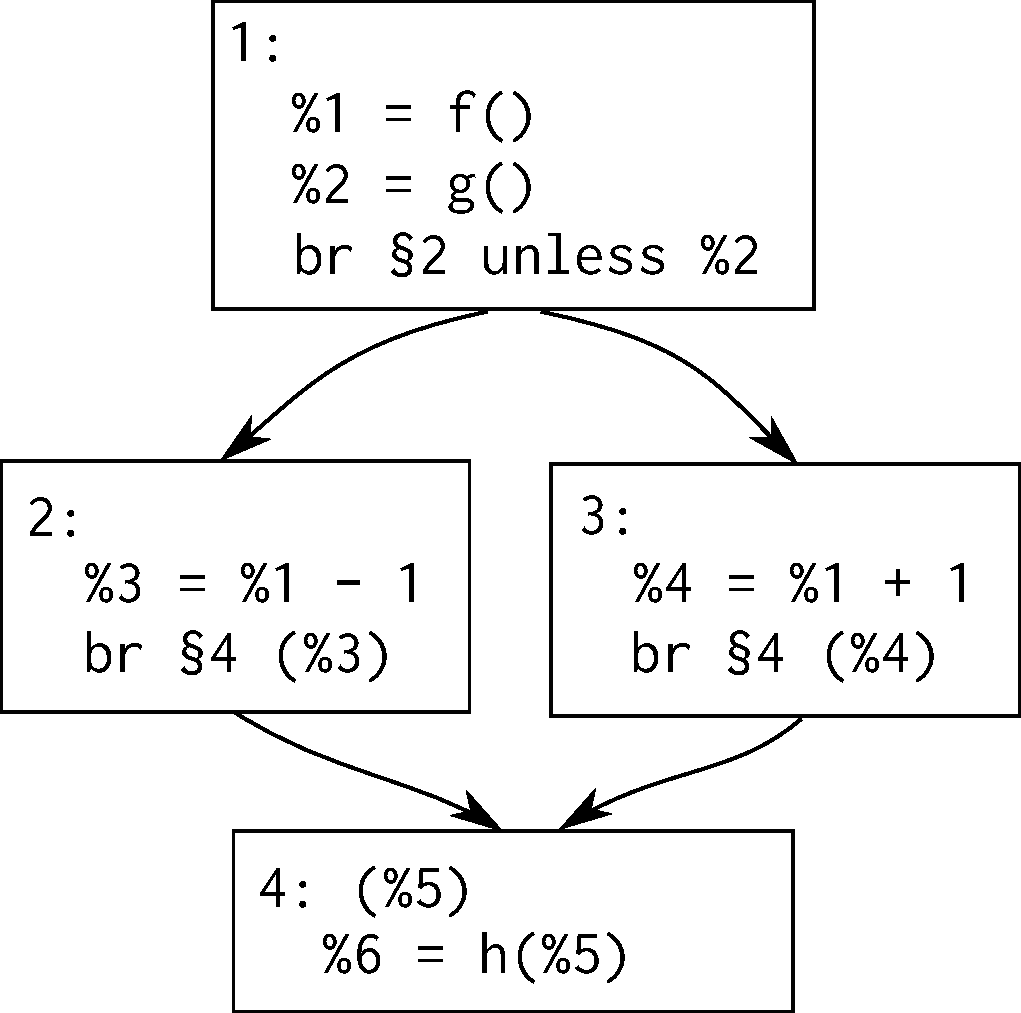
\includegraphics[width=0.4\textwidth]{figures/ssa-args}}
  \hfill\null
  \caption{Two control flow graphs of the same function, illustrating the correspondence between SSA
    representations using \(\phi\)-functions and block arguments.  The SSA variables
    \protect\jlinl{\%3} and \protect\jlinl{\%4} correspond to the values of \protect\jlinl{y} in the
    two branches, which are merged in \protect\jlinl{\%5}.}
  \label{fig:ssa-phi}
\end{figure}

Note that until now, the operations involved were purely syntactic in nature, and could be performed
by solely taking into account the code of the function \jlinl{foo}.  As soon as \jlinl{foo} is
called on a concrete type during evaluation, though, the most specific method fitting to the
argument types will be selected, and type inference on its body be applied.  If we go on and call
\jlinl{foo([1.0])}, with \jlinl{Vector\{Int\}} as the sole argument type, the types as annotated in
the same listing will be inferred.

\begin{lstfloat}[p]
  \begin{lstlisting}[style=lstfloat]
1 ── %1  = arraysize(x, 1)::Int64
│    %2  = slt_int(%1, 0)::Bool
│    %3  = ifelse(%2, 0, %1)::Int64
│    %4  = slt_int(%3, 1)::Bool
└───       goto §3 if not %4
2 ──       goto §4
3 ──       goto §4
4 ┄─ %8  = φ (§2 => true, §3 => false)::Bool
│    %9  = φ (§3 => 1)::Int64
│    %10 = φ (§3 => 1)::Int64
│    %11 = not_int(%8)::Bool
└───       goto §22 if not %11
5 ┄─ %13 = φ (§4 => 0.0, §21 => %18)::Float64
│    %14 = φ (§4 => %9, §21 => %42)::Int64
│    %15 = φ (§4 => %10, §21 => %43)::Int64
│    %16 = arrayref(true, x, %14)::Float64
│    %17 = invoke sin(%16::Float64)::Float64
│    %18 = add_float(%13, %17)::Float64
│    %19 = sle_int(1, 1)::Bool
└───       goto §7 if not %19
6 ── %21 = sle_int(1, 0)::Bool
└───       goto §8
7 ──       nothing::Nothing
8 ┄─ %24 = φ (§6 => %21, §7 => false)::Bool
└───       goto §10 if not %24
9 ──       invoke getindex(()::Tuple, 1::Int64)::Union{}
└───       $(Expr(:unreachable))::Union{}
10 ┄       goto §11
11 ─       goto §12
12 ─       goto §13
13 ─       goto §14
14 ─ %32 = invoke :(var"#sprint#339")(
             nothing::Nothing, 0::Int64, sprint::typeof(sprint), 
             show::Function, %18::Float64
           )::String
└───       goto §15
15 ─       goto §16
16 ─       goto §17
17 ─       invoke println("y += sin(x[i]) = "::String, %32::String)::Any
│    %37 = (%15 === %3)::Bool
└───       goto §19 if not %37
18 ─       goto §20
19 ─ %40 = add_int(%15, 1)::Int64
└───       goto §20
20 ┄ %42 = φ (§19 => %40)::Int64
│    %43 = φ (§19 => %40)::Int64
│    %44 = φ (§18 => true, §19 => false)::Bool
│    %45 = not_int(%44)::Bool
└───       goto §22 if not %45
21 ─       goto §5
22 ┄ %48 = φ (§20 => %18, §4 => 0.0)::Float64
└───       return %48
\end{lstlisting}
  \caption{Typed and optimized code of the call \protect\jlinl{foo([1.0])} in SSA form, as obtained
    through \protect\jlinl{@code_typed} (the extra bars are due to the formatting of
    \protect\jlinl{CodeInfo}).\label{lst:foo-typed}}
\end{lstfloat}

The last step of compilation within Julia consists of inlining and optimizing the typed intermediate
code, resulting in the form shown in listing~\ref{lst:foo-typed}.  There, several called methods
have been inlined, and concrete argument types to invoke been inferred.  This is in true,
traditional SSA form, with all variable slots eliminated, and block arguments converted to the
mentioned \(\phi\)-functions.  Finally, this representation will be translated and sent to LLVM for
compilation, where further optimization can happen, and machine code will be generated and executed,
as well as stored for later usage as part of the just-in-time compilation mechanism.

\newthought{A key principle} in Julia's compilation model is type specialization
\parencite{bezanson2018julia}.  As we have seen, whenever a function call is evaluated, the types of
the arguments are first determined, and then the most specific method selected and called.  This
automatically gives the language dynamic semantics: an implementation can perform evaluation at
every call.  In practice, however, at this point multiple dispatch and JIT compilation combine into
one of the main principles of optimization.  Instead of evaluating the same code over and over
again, methods are JIT-compiled the first time they are called.  The compiled code is then cached in
the method table.  Method compilation does not happen recursively at once, though.  Only when the
body of a compiled method is then executed with concrete arguments, the same process is performed
again, for each invoked method.

So, in a sense, JIT compilation can be seen as a function that returns compiled code, given a
function and a tuple of types.  Similar to macros, which transform original code, given an
expression, this process of generating compiled methods from types is customizable in Julia: via
so-called \emph{generated functions}, there exists a process to dynamically generate code, given
argument types~-- a form of staged programming
\parencite{rompf2010lightweight,bolewski2015staged}. Such generated functions, when called, are not
directly translated into machine code: instead, they emit new code to the compiler, based on the
types of their arguments.  The new code is then JIT-compiled.  For example, when we have two methods
of a function \jlinl{f}:
\begin{lstlisting}
f(x::Int) = println("Int")
f(x::String) = println("String")
\end{lstlisting}
we could replace them with the following generated function:
\begin{lstlisting}
@generated function f_generated(x)
    if x == Int
        return :(println("Int"))
    elseif x == String
        return :(println("String"))
    else
        error("Method error")
    end
end
\end{lstlisting}
Calling \jlinl{f_generated(1)} will then determine the argument type (\jlinl{typeof(1) == Int}), and
pass it to the function body of \jlinl{f_generated}.  There, the conditional will select the first
branch, and the expression \jlinl{:(println("Int"))} be returned.  This is now passed back to the
compiler, which will lower the code and compile the method for \jlinl{Int} arguments, and store the
result in the method table.  The stored code can then be executed~-- on the arguments that were used
to determine the type tuple the generated function has been called with!  The next time
\jlinl{f_generated} is executed, the function body is \emph{not} executed anymore, but the generated
code of the the function defined through the expression \jlinl{:(println("Int"))} directly looked
up\footnote{A caveat: technically, the compiler is still free to call the generating code multiple
  times~-- which is the reason generated functions should never involve side effects or depend on
  external state.}.  Of course, simply replacing dispatch, as with this example, is not what
generated functions are used for in practice.  Most applications concern parametric types with
statically known shape arguments, such as tuples, named tuples, or array ranks.  They can also be
used for type-level computations on values that become known only known at run-time, through
singleton types such as \jlinl{Val}.

The direct generation of code, given argument types, is however not the furthest we can go.  For
one, generated functions are not only allowed to return \jlinl{Expr} objects~-- the internal
representation of the surface AST~-- but also \jlinl{CodeInfo} objects, which are the internal
representation of lowered code in (almost) SSA form.  This, on its own, would not be of much use
most times, but there is a second, more interesting feature: it is possible to query the
\jlinl{CodeInfo} of a method by reflection, given a function and an argument type tuple.  Combining
these two, we now have all the tools to implement IR-level code transformations as follows:
\begin{enumerate}
  \firmlist
\item Define a generated function, taking as arguments another function and its arguments.
\item Within this function, obtain the IR of the method of the passed-in function for the remaining
  arguments.
\item Transform this IR however necessary.
\item Return the IR, which will now be compiled and called on the actual arguments.
\end{enumerate}
Importantly, unlike macros, such transformations can be performed \emph{recursively}: one simply
inserts the same generated function to inner function calls during the transformation in step 3.
Since the transformation operates not during parsing, the function to be transformed needs not be
known beforehand, and not be present literally in the code~-- the generated function can be called
on every available callable object, at any time during run-time.  This makes it possible to transform
even functions from other libraries, internally calling yet other functions.  One particular example
of this principle is source-to-source automatic differentiation, as shown in the next chapter: a
call to a function \jlinl{gradient(f, x, y)} will obtain the IR of the method for \jlinl{f} on
\jlinl{typeof(x)} and \jlinl{typeof(y)}, produce differentiated code, and call the result on
\jlinl{x} and \jlinl{y}.  Naturally, differentiating \jlinl{f} involves recursively differentiating
the other, unknown functions within it, too (down to \enquote{primitive} functions, whose derivative
is known), and combining the results using the chain rule.

This metaprogramming pattern is extremely powerful, and becoming more and more popular.  It allows
to change evaluation semantics in more profound ways than multiple dispatch can: by rewriting the
code of the called function, it is possible to change what invoking a method within its body means.
Through this, several abstract interpretation algorithms can be realized, by extending the existing
data path with additional metadata (such as automatic differentiation, or other forms of information
propagation analysis \parencite[part II]{singer2018static}), or non-standard execution be
implemented (e.g., continuation-passing style transformations).  There exist already two Julia
packages with the goal of simplify working with this kind of transformation:
\juliapackage{Cassette.jl}\footnote{\protect\url{https://github.com/jrevels/Cassette.jl}}, which
provides overloadable function application by a so-called \enquote{overdubbing} mechanism,
abstracting out some common patterns; and
\juliapackage{IRTools.jl}\footnote{\protect\url{https://github.com/FluxML/IRTools.jl}}, which has a
more user-friendly alternative to \jlinl{CodeInfo}, and a macro similar to \jlinl{@generated} that
makes writing recursive functional IR-transformation using this data structure easier.  The latter is
what the work of this thesis builds on.


%%%%%%%%%%%%%%%%%%%%%%%%%%%%%%%%%%%%%%%%%%%%%%%%%%%%%%%%%%%%%%%%%%%%%%%%%%%%%%%%%%%%%%%%%%%%%%%%%%%
\section[Automatic Differentiation and Computation Graphs]{Automatic Differentiation and \newline
  Computation Graphs}
\label{sec:cg-ad}

This section may appear as an outlier from the original topic; in fact, the mathematics developed
here are not even used later.  However, it is important to explain the interrelations between
automatic differentiation (AD), computation graphs, and IR transformations, to be able to understand
how SSA-form representation is a natural structure for extracting and analyzing computation graphs,
and how the necessary transformations arise in practice.  To appreciate how the form of the
computation graphs interacts with the mathematics, some foundations need to be introduced first.

\newthought{Many algorithms in machine learning} and other domains can be expressed as an
optimization problem over a multivariate function with scalar output~-- typically a loss function
over a parameter space, which measures how far a model prediction is form the true target values.
The optimal model is then just that one for which the parameters minimize the loss function.  When
the loss function is (sub-)differentiable, there exist a variety of gradient-based optimization
methods to find this optimum (or, in the non-convex case, at least a practically sufficient local
minimum).

While in some cases the loss function is simple enough to find the gradient by hand, in general, the
model, and therefore the loss function, may be specified in terms of rather complicated programs,
for which hand-writing derivatives is difficult to infeasible.  For this reason, computerized
methods for differentiation have been developed.  These can be categorized into three classes:
\begin{itemize}
  \firmlist
\item Finite differences
\item Symbolic differentiation
\item Automatic differentiation
\end{itemize}
In finite differences, the idea is to discretize the definition of derivatives, and numerically
evaluate the function within an environment.  This is simple to implement, but does not scale well
with the dimension of the involved space, and can become numerically unstable in various ways
\parencite[section 5.7]{press2007numerical}.  Symbolic differentiation works through representing
the functions in question as symbolic algebraic objects, and applying the differentiation rules as
one would manually.  This does not lose precision or introduce divergence, but can suffer from
blow-up of the size of the generated expressions; additionally, it requires the functions to be
expressed in a custom representation, different from normal functions or programs
\parencite{baydin2018automatic}.

\newthought{Automatic differentiation}, the third category, is perhaps unfortunately named~-- it
does not signify much at first sight.  The relevant idea is to not start from functions as black-box
or symbolic objects, but from programs.  Then the perturbation that makes up the value of the
derivative at a point is propagated through the steps of the program.  For this to work, there needs
to exist an explicit representation of the computation graph at  the evaluation at a point, which
is what makes the topic relevant for this thesis.  In contrast to the former two methods, AD relies
on numeric, not symbolic evaluation, but is (up to the floating point errors already present in the
input function) exact~-- no discretization error, as in finite differences, is introduced.  For a
more detailed treatment, I refer to \textcite{griewank2008evaluating}, the standard work on the
topic, and the survey by \textcite{baydin2018automatic}, which includes a comparison of
state-of-the-art implementations.  There are many works on the formalization of AD in programming
language theory; see, for example, \textcite{abadi2020simple}.

To understand how AD works, let us first start with the mathematics.  What is a derivative, really?
When we talk about gradients, which is what we really need in a gradient algorithm, this is usually
a rather informal term for \enquote{the vector of partial derivatives}, which then points into an
ascent direction.  This is however not the most natural form to work with in a compositional
approach.  Instead of starting with a limit of tangent slopes, more insight is provided by viewing
derivatives as best-approximating linear operators.  One of the most general definitions is provided
through the \emph{Fréchet derivative} \parencite[p. 463]{bronstein1995taschenbuch}, essentially a
generalization of the total differential.  Let \(X\) and \(Y\) be normed spaces.  A function
\(f: U \subseteq X \to Y\) is Fréchet differentiable at a point \(x \in U\) if there exists a
bounded linear operator \(A: X \to Y\) such that
\begin{equation}
  \label{eq:frechet}
  \lim_{\enVert{\Delta}_X \to 0} \frac{\enVert{f(x + \Delta) - f(x) -
      A(\Delta)}_Y}{\enVert{\Delta}_X} = 0.
\end{equation}
When such an \(A\) does exist, it is unique, and we may call it \emph{the} derivative of \(f\) at
\(x\), writing \(\Dif f(x) = A\).  When the derivative exists for all \(x\), we can use \(\Dif\) as
a well-defined higher-order function on its own; we will assume this in the following.\footnote{In
  in practical cases, functions are often only piecewise differentiable due to branches, failing
  this definition on a countable set of points.  Fortunately, the formalism of AD remains the same
  under weaker notions of differentiability.  Additionally, such points usually behave well enough
  to admit a subdifferential, from which we can just choose an arbitrary subgradient; this does not
  necessary lead to a descent direction, but still allows minimization under reasonable conditions
  \parencites[see][section 6.1]{pock2017convex}[][chapter
  14]{griewank2008evaluating}{abadi2020simple}.}

The important fact here is that \(\Dif f(x)\) is still a function: specifically, a linear function
approximating how \(f\) reacts to an input perturbation, \(\Delta\), around \(x\).  Or, in other
words:
\begin{equation}
  f(x + \Delta) = f(x) + \Dif f(x)(\Delta) + o\left(\enVert{\Delta}\right).
\end{equation}
This fact allows one to propagate differential values through composed functions, by the chain rule,
which we write in the following compositional form:
\begin{equation}
  \Dif(\phi \circ \psi)(x) = \Dif\phi(\psi(x)) \circ \Dif\psi(x).
\end{equation}
In the one-dimensional case, we simply have
\begin{equation}
  \Dif \phi(x) = \Delta \mapsto \partial_1 \phi(x) \, \Delta,
\end{equation}
where \(\partial_1 \phi(x)\) denotes the standard \enquote{primitive} derivative, since linear maps
are exactly multiplications by a scalar.  Therefore, we can recover the chain rule
\begin{equation}
  \begin{aligned}
    \Dif(\phi \circ \psi)(x)(\Delta) &=
    \left( \Dif\phi(\psi(x)) \circ \Dif\psi(x) \right)(\Delta) \\
    % &= \Dif\phi(\psi(x))\left( \Dif\psi(x)(\Delta) \right) \\
    % &= \Dif\phi(\psi(x))\left( \partial_1 \psi(x) \, \Delta \right) \\
    % &= \partial_1\phi(\psi(x)) \, \partial_1 \psi(x) \, \Delta \\
    &= \left( \partial_1\phi(\psi(x)) \, \partial_1 \psi(x) \right) \, \Delta,
  \end{aligned}
\end{equation}
as we know it from calculus.  Here, the product in the resulting expression arises from the fact
that we propagated through \(\partial_1 \psi(x) \Delta\) as the input value of
\(\Dif\phi(\psi(x))\).  It is, however, remarkable that this formula is not entirely compositional:
to construct \(\Dif(\phi \circ \psi)\), it is not only necessary to know \(\Dif\phi\) and
\(\Dif\psi\), but also \(\psi\) \parencite{elliott2018simple}.  Still, this is not as bad as it may
seem: as I will now explain, AD algorithms evaluate both \((\phi \circ \psi)(x)\) and
\(\Dif(\phi \circ \psi)(x)\) at once, in lockstep fashion, so that the intermediate values of the
former can be reused in calculation of the latter.

Consider the specific case of \(f(x, y) = sin(x) - y\). For simpler notation, let
\(g = (x, y) \mapsto x - y\) replace the infix subtraction operator, with a derivative of
\(\Dif g(x)(\Delta_1, \Delta_2) = \Delta_1 - \Delta_2\).  By composition, we have:
\begin{equation}
  \begin{aligned}
    \Dif f(x, y) &= \Dif(g \circ (\sin \otimes \ident))(x, y) \\
    &= \Dif g\left( (\sin \otimes \ident)(x, y) \right) \circ \Dif(\sin \otimes \ident)(x, y) \\
    % &= \left( (\Delta_1, \Delta_2) \mapsto \Delta_1 - \Delta_2 \right) \circ \left( \Dif\sin(x)
      % \otimes \Dif \ident(y) \right) \\
    % &= (\Delta_1, \Delta_2) \mapsto \partial_1\sin(x) \, \Delta_1 - 1 \Delta_2 \\
    &= (\Delta_1, \Delta_2) \mapsto \cos(x) \, \Delta_1 - \Delta_2.
  \end{aligned}
\end{equation}
In order to calculate this algorithmically, let us expand the computation of \(f\) into a sequence
of intermediate, primitive calculations, as we would have in a programmatical representation:
\begin{equation}
  \label{eq:ad-primal}
  \begin{aligned}
    x &= \operatorname{?}, \\
    y &= \operatorname{?}, \\
    z &= \sin(x), \\
    \Omega &= g(z, y).
  \end{aligned}
\end{equation}
We have given the final result the name \(\Omega\), and and introduced an intermediate value \(z\).
This is known as the \emph{forward}, or \emph{primal} function in AD terminology.  The relations of
these values can be expressed as the black computation graph in figure~\ref{fig:comp-graph-fw}.
Following the graph, or equivalently, following the equations in ~\eqref{eq:ad-primal}, the
composition of the derivative operators can be built up incrementally, as shown in the blue part of
that figure, by calculating the following \emph{tangent values}:
\begin{equation}
  \label{eq:ad-forward}
  \begin{aligned}
    \dot{x} &= \Delta_1, \\
    \dot{y} &= \Delta_2, \\
    \dot{z} &= \Dif\sin(x)(\dot{x}) \\
    &= \cos(x) \, \Delta_1, \\
    \dot{\Omega} &= \Dif g(z, y)(\dot{z}, \dot{y}) \\
    &= \cos(x) \, \Delta_1 - \Delta_2.
  \end{aligned}
\end{equation}
The tangent values of input variables \(x\) and \(y\) become the input perturbations \(\Delta_i\).
For every subsequent tangent value, we apply the derivative at the corresponding primal variable
(depending on the primal parents) to the tangent values of the parents~-- this way, the composition
of the derivative operators follows the chain rule.  This algorithm, called \emph{forward-mode AD},
can now be applied practically not only on symbolic functions, but on programs, by always jointly
computing \((v, \dot{v})\) for every variable \(v\), given its parents in the graph.  This requires
a form of non-standard execution, which will be explained in more detail below.

\begin{figure}[t]
  \centering
  \subbottom[Forward mode.\label{fig:comp-graph-fw}]{%
    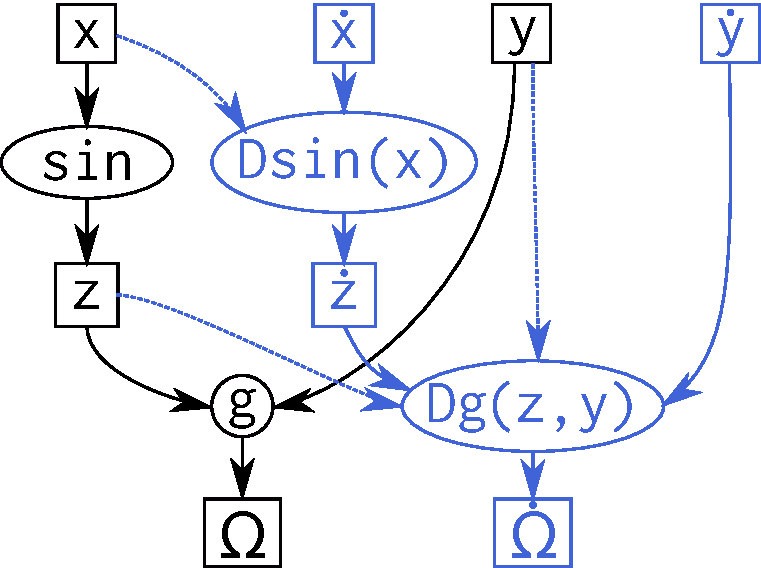
\includegraphics[]{figures/comp-graph}}
  \qquad
  \subbottom[Backward mode.\label{fig:comp-graph-bw}]{%
    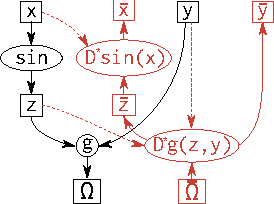
\includegraphics[]{figures/comp-graph-backward}}
  \caption{Computation graph and intermediate expressions of the expression \protect\jlinl{g(sin(x),
      y)}, together with the derivative graphs in forward- and backward mode.  Dashed arrows
    indicate re-use of primal values in the derivative graph.}
  \label{fig:comp-graph}
\end{figure}

\newthought{Recovering the full gradient} of a function \(\phi: U \subseteq \RR^N \to \RR\) (which
is generally the form of loss functions for parametric models) requires to evaluate \(\Dif \phi(x)\)
\(N\) times, however.  This is because individual partial derivatives can only be extracted from
\(\Dif \phi(x)\) by calculating the sensitivities to unit input perturbations in coordinate
directions, for each of the input variables:
\begin{equation}
  \nabla \phi(x) = \begin{pmatrix}
    \Dif \phi(x)(1, 0, \ldots, 0)  \\
    \vdots \\
    \Dif \phi(x)(0, \ldots, 0, 1)
  \end{pmatrix} = \begin{pmatrix}
    \partial_1 \phi(x) \\
    \vdots \\
    \partial_N \phi(x)
  \end{pmatrix},
\end{equation}
which is really a special case of taking directional derivatives (which can be recovered generally
by application of the differential to any vector with unit norm.)

In order to overcome the increase of complexity with the number of input dimensions, we can
reformulate the compositional equation.  Let us introduce \(\CoDif \phi(x)\), the \emph{adjoint
  operator} of \(\Dif \phi(x)\), whose defining property is that in \enquote{inverts} the order of
the perturbation application: instead of calculating a primal sensitivity with respect to an input
perturbation (\(\Delta\)), it maps a linear output perturbation (\(\mathfrak{d}\)) to an operator
that applies this to the primal sensitivity:
\begin{equation}
  \CoDif \phi(x)(\mathfrak{d}) = \Delta \mapsto \mathfrak{d}(\Dif \phi(x)(\Delta)).
\end{equation}
The adjoint differential is therefore an object of the double dual space.  This becomes more
readable when we fix a basis to represent the derivative.  Doing so, in the finite-dimensional case,
the derivative \(\Dif \phi(x)\) is the Jacobian matrix at \(x\), \(J_{\phi}(x)\).  In this setting,
forward-mode AD is simply an efficient way to calculate the \emph{Jacobian-vector-product}
\(J_{\phi}(x) \Delta\), or equivalently the total derivative for a fixed perturbation, avoiding full
matrix multiplication~-- which is the reason we have to apply it to the basis vectors to get back
the gradient.  Backward mode, on the other hand, calculates the product of the Jacobian with the
operator that should be applied to the result, but does not yet apply it to the input
perturbation~-- therefore, it returns a matrix:
\begin{equation}
  \begin{aligned}
    \mathfrak{d} (\Dif \phi(x)(\Delta)) &= \transpose{d} J_{\phi}(x) \Delta \\
    &= \transpose{\left( \transpose{J_{\phi}(x)} d \right)} \Delta \\
    &= \CoDif \phi(x)(\mathfrak{d})(\Delta),
  \end{aligned}
\end{equation}
where we assume \(\mathfrak{d}\) to be represented by the co-vector \(\transpose{d}\).  Since the
unapplied \(\CoDif \phi(x)(\mathfrak{d})\) is itself an object in the dual space, it is also
represented as a co-vector~-- and in fact, nothing else than a transformation of the transposed
Jacobian.  Recovering the gradient of a loss function then reduces to evaluating it at a constant
scalar output perturbation of \(1\), which is equivalent to the application of the primal
differential to the matrix of basis vectors.

Note that due to this relation to the transpose, the adjoint operator inverses the order of
composition in the chain rule:
\begin{equation}
  \begin{aligned}
    \CoDif (\phi \circ \psi)(x)(\mathfrak{d}) &= \transpose{d} J_{\phi}(\psi(x)) J_{\psi}(x) \\
    &=  \transpose{\left( \transpose{J_{\psi}(x)} \transpose{J_{\phi}(\psi(x))} d \right)} \\
    &= \left( \CoDif\psi(x) \circ \CoDif\phi(\psi(x)) \right)(\mathfrak{d}).
  \end{aligned}
\end{equation}
For our example function \(f\), this gives the same structural form of the result as the forward
mode~-- only that now, the value is a vector:
\begin{equation}
  \begin{aligned}
    \CoDif f(x, y) &= \CoDif (g \circ (\sin \otimes \ident))(x, y) \\
    &= \CoDif(\sin \otimes \ident) \circ \CoDif g((\sin \otimes \ident)(x, y)) \\
    % &= (\CoDif\sin \otimes \CoDif\ident) \circ (\delta \mapsto \transpose{[\delta, -\delta]}) \\
    % &= (\partial_1 \sin(x) \otimes 1) \circ (\delta \mapsto \transpose{[\delta, -\delta]}) \\
    % &= \delta \mapsto \transpose{[\partial_1\sin(x)\delta, -1 \delta]} \\
    &= \delta \mapsto \transpose{[\cos(x)\delta, -\delta]}.
  \end{aligned}
\end{equation}
In this form, starting with an output perturbation \(\delta = 1\), we get back the gradient tuple
through just one evaluation.  Incidentally, this is nothing else than the back-propagation
\enquote{trick} \parencite{bishop2006pattern}!  Furthermore, applying this result to
\([\Delta_1, \Delta_2]\) gives back the linear combination of the forward mode result.

In programmatic terms, we can proceed similar to above, only this time introducing \emph{adjoint}
intermediate values \(\bar{v}\).  For the values in equation~\eqref{eq:ad-primal}, we get
\begin{equation}
  \label{eq:ad-backward}
  \begin{aligned}
    \bar{x} &= \bar{z}_2 = -\delta, \\
    \bar{y} &= \CoDif\sin(x) \, \bar{z}_1 \\
    &= \cos(x) \, \delta\\
    \bar{z} &= \CoDif g(x, y)(\bar{\Omega}) \\
    &= [\delta, -\delta] \\
    \bar{\Omega} &= \delta,
  \end{aligned}
\end{equation}
which is displayed in the red graph in \ref{fig:comp-graph-bw}.  Note that now, the back-propagated
values can not be computed in parallel with forward evaluation; hence the equations are stated in
reverse order.  Instead, the intermediate primal values have to be remembered and reused in a
second, backward pass.

Finally, it has to be noted that the two described modes of automatic differentiation are only two
extremes of a spectrum.  Forward and backward calculations can really be interleaved in arbitrary
order, just as it is possible to multiply Jacobians and their transposes in different order.  One
frequent use case of this \emph{mixed-mode AD} is when loss functions, differentiated using backward
mode, contain broadcasting functions; for example, nonlinearities in neural network.  These have a
shape of \(\RR^N \to \RR^N\), but only involve a linear number of operations, so forward mode pays
off\footnote{As a rule of thumb in Julia, for \(f: \RR^M \to \RR^N\), forward mode typically
  performs better when \(M \ll N\) or as long as \(M \lessapprox 100\).  This folklore should always
  be confirmed by benchmarking, though.  See
  \url{https://github.com/JuliaDiff/ReverseDiff.jl\#should-i-use-reversediff-or-forwarddiff}.}.
Similar properties hold for second order derivatives: the calculation of Hessians is often fastest
by using forward-over-reverse composed differentiation.  In general, unfortunately, determining the
optimal order of derivative evaluation is hard~-- this so-called \emph{optimal Jacobian
  accumulation} problem is known to be NP-complete \parencite{naumann2007optimal}.

\newthought{The practical implementation} of automatic differentiation in programming languages
opens up another set of possible choices.  One way is to use an external, compiler-based system that
transforms a complete program in a subset of a standard programming language (e.g., Tapenade, which
transpiles Fortran and C code \parencite{tapenadedevelopers2019tapenade}) or in a custom
specification, as is done in Stan \parencite{carpenter2015stan}.  But both of these examples are
really applied in niche cases: large numeric simulations, and log-densities in a probabilistic
model.  These systems lack flexibility in programming, especially concerning abstractions and
interaction with other libraries, and require external tooling besides a main programming language.
Recently, the Swift for TensorFlow project \parencite{tensorflowdevelopers2018swift,hong2018graph}
introduced a modern variant of this by extending the compiler of the Swift programming language with
facilities to perform automatic differentiation internally, and some features to simplify graph
operations required by TensorFlow.

The second possibility is \emph{operator overloading}.  Forward mode can be recast in mathematically
equivalent form by using dual numbers \parencite[see][section 3.1.1]{baydin2018automatic}.  These
consist of two parts, similar to complex numbers: \(z = x + y\epsilon\).  However, contrary to the
imaginary unit, the infinitesimal unit \(\epsilon\) vanishes under multiplication with itself:
\(\epsilon^2 = 0\).  The consequence of this is that functions can naturally be extended to dual
numbers by nonstandard interpretation as truncated Taylor series:
\begin{equation}
  \phi(x + \epsilon) = \phi(x) + \partial_1\phi(x)\epsilon + \underbrace{\frac{\partial^2_1\phi(x)}{2}\epsilon^2
  + \ldots}_{\epsilon^2 (\ldots) = 0}
\end{equation}
Since the higher order terms vanish, this is exactly the tuple of primal and tangent value that is
calculated during the lockstep evaluation in forward mode:
\begin{equation}
  (z, \dot{z}) = (\phi(x), \Dif\phi(x)(\dot{x})) \quad\Leftrightarrow\quad z + \dot{z}\epsilon = \phi(x + \dot{x}\epsilon).
\end{equation}
(generalization to higher dimensions, as well as higher derivatives in form of hyper-dual numbers,
follow equally naturally.)

Dual numbers can rather easily be added to an existing programming language that has a sufficiently
extensible system for overloading mathematical operators.  This can be done using traits or type
classes, like in Haskell, or by dynamic dispatch, which is what is used in Python and Julia.  The
latter is especially versatile in this respect, since every function can be extended to a new type
of dual numbers by simply adding a method; unlike in Python, where only certain operators are open
to extension~-- a fundamental limitation of its single dispatch, object oriented approach.

\begin{figure}[t]
  \centering
  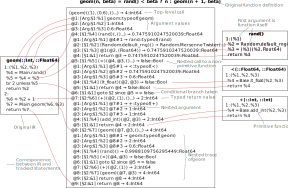
\includegraphics{figures/wengert-list}
  \caption{Wengert list of the example function \protect\jlinl{g(sin(x), y)} introduced above.
    Every intermediate variable becomes an element, linked through pointers.  The gradient can be
    calculated by backward traversal and accumulating the adjoint values as metadata in the list
    elements.}
  \label{fig:wengert-list}
\end{figure}

Backward-mode AD can be implemented using operator overloading as well, but this requires more
effort.  Since adjoint values cannot be simply threaded through in parallel to forward evaluation,
one needs to build up a data structure during the forward pass, which can at the end be traced back
in reverse order.  One possibility of doing this is to use closures, but the usage of many higher
order function might lead to unwanted heap allocation and makes understanding harder.

The alternative is to use a tape structure, or \emph{Wengert list} \parencite[][section
3]{baydin2018automatic}.  On such a list, the computation graph is stored as by pointers between
elements, as shown in figure~\ref{fig:wengert-list}.  The Wengert list can also be constructed
through an operator overloading approach, which is exactly what graph-based machine learning
frameworks do: PyTorch \parencite{paszke2017automatic}, TensorFlow \parencite{abadi2015tensorflow}
in eager mode, DyNet \parencite{neubig2017dynet}, and Chainer \parencite{tokui2015chainer}.  In
these, the programmer interacts with a library mirroring the usual numerical functions, but
operating on a special \enquote{variable} or \enquote{tensor} type.  These operations are overloaded
so that function calls, in addition to performing the primal calculations, are stored either
explicitly on a global Wengert list structure, or implicitly in the constructed expression objects.
Then, one can start a backward pass from any leaf variable to propagate back derivatives to the
roots of the computation graph, by following the edges and summing up adjoint values in parent
nodes' metadata.  JAX \parencite{bradbury2018jax} carries the idea further and allows general
composable source transformations to implement not only differentiation, but also vectorization,
parallelization, and other syntactic abstractions over functional programs written in Python, over a
unified intermediate representation that is recovered from an original function by tracing.

This style of implementation has limitations, though: it requires building up many objects at
run-time, and is completely oblivious of control structures.  Additionally, the code expressing
differentiable functions has to be written entirely in the DSL, in a library-aware fashion,
preventing the usage of third-party functions and language features, and forcing the user to adhere
to certain semantic constraints that cannot be verified statically by the host language.  TensorFlow
in graph mode addresses some of these points.  It builds up a complete expression graph, which is
differentiated symbolically, and is therefore somewhat in the middle between operator overloading
(since the graph is still a run-time data structure) and a static transformation (the resulting graph
is not interpreted in the host language, but converted to run on an \enquote{accelerator}, which can
one of several kinds of processing unit~-- CPU, GPU, TPU,\ldots).  It still requires to stick to the
provided expression types and library functions, though.

Efforts to overcome these limitations lead to the third kind of approach: language-internal
\emph{source transformation}.  Recent work in Julia \parencite{innes2018don} has shown that through
the available metaprogramming mechanisms (described in section~\ref{sec:comp-metapr-julia}) allow to
systematically derive \enquote{adjoint programs} for arbitrary user-provided Julia functions, given
only an extensible set of \emph{primitive adjoints}.  This approach works purely structurally on the
Julia IR, employing generated functions to analyze functions' code and transform them completely,
including third-party functions and data types, and control flow.  The key insight here is that
SSA-form IR already resembles the structure of Wengert lists, extended by branches.  As in building
up reverse computation graphs, the adjoint code will therefore invert the control flow of the basic
blocks in the primal function, taking into account that data flow may involve dynamic dependencies.
Differentiation through data types and closures is supported via a unified treatment of them in a
tuple-like form, with constructors and accessors (inspired by cons-cells in Lisp).

An implementation of this principle has been released as the \juliapackage{Zygote.jl}
package\footnote{\url{https://github.com/FluxML/Zygote.jl}}.\todo{list some code\_adjoint output?}
In similar spirit, there is also work on directly differentiating the LLVM intermediate
representation, by extending the compiler pipeline with a differentiation pass that comes after all
language-specific and high-level optimizations \parencite{moses2020instead}.  Furthermore, there are
applications that use the same techniques for other purposes, like sparsity detection
\parencite{gowda2019sparsity} or concolic execution \parencite{churavy2019vchuravy}.  

Internal source-based methods can therefore be composable, extensible, and more user-friendly, since
no special treatment of programs to be differentiated is required: primal functions can be
implemented as any other regular function in the host language.  A source-transformation approach
also completely avoids the obscure issue of \enquote{perturbation confusion}, which leads to
hard-to-find errors when using nested differentiation with dual numbers
\parencite{baydin2018automatic,manzyuk2019perturbation}.

As a concluding note, all these graph operations reveal that automatic differentiation is really
only a special case of message passing algorithms in computation graphs
\parencite{minka2019automatic}.  Other learning methods that can be described as message passing are
optimization algorithms \parencite{ruozzi2011message,dauwels2005steepest} and a variety of
variational approximations \parencite{winn2005variational,minka2005divergence}.  Hence, it is no
surprise that computation graphs play a large role as the foundation of other learning algorithms in
Bayesian methods, such as described below.

%%% Local Variables: 
%%% TeX-master: "main"
%%% End:
\chapter{Implementation of Dynamic Graph Tracking in Julia}
\label{cha:impl-dynam-graph}

As we have seen, there is a trade-off between source-transformation methods and library-based
approaches for tracking computation graphs.  Since the ultimate goal of this work was to target
dynamic probabilistic models written in \turingjl{}, properties of both were derired.  Inspired the
the work of \textcite{innes2018don}, it seemed most promising to start with a source-transformation
based approach implemented over the intermediate representation, especially from a usability point
of view.  However, the dynamicity of the trace structure of general probabilistic programs needes to
be preserved.  Hence, I developed an idea for a hybrid version: through an IR transformation, the
original code of a function to be tracked should be exteded by additional statements to record a
trace of the executed statements and control flow operations at runtime.  The algorithm and data
structure on which this implementation is based have already been shortly described in
\textcite{gabler2019graph}, and will be more extensively explained below.


\section{Extended Wengert Lists}
\label{sec:exteded-wengert-lists}

We have seen above, in section~\ref{sec:comp-metapr-julia}, how generated functions allow inspection
and transformation of the intermediate representation passed-in functions.  This technique can be
applied to recursively traverse the implementation of a given function, annotating each operation
with necessay tracking statements, and changing the inputs and outputs accordingly to extract this
information from outside.  To ensure sufficient generality, we requite the following properties of
the tracking system:
\begin{enumerate}
\item Literal capture expressions and branches in an analyzable, graphical form.
\item Preservation of the relation of each part of the structure to the corresponding original IR.
\item Proper nesting of this information for nested function calls, making relations between
  arguments and function inputs recoverable.
\item Correct handling of constants and primitive functions in the IR.
\item Extensibility of the tracking functions, to allow multiple possible ways to analyze code
  (e.g., by different definitions of what should be recorded).
\item A way to add custom metadata to the recorded structure turing tracking.
\end{enumerate}
This kind of operation will be similar to the (explicit) construction of Wengert lists in
backwards-mode AD; but contrary to there, the nested call structure and control flow shall be
preserved as well.  Hence, we call this structure \emph{extended Wengert list}.



% Figure 1 illustrates the extended Wengert list for one run of a short stochastic function
% geom (for readability, it is expanded to only three levels). The geom function draws a sample
% from the geometric distribution with parameter beta, starting to count at value n. On
% the left, we have its IR in textual form, consisting of two blocks. The central part is the
% graph of nested nodes. There, values and jumps from the top-level call are recorded in their
% encountered order, as nodes with “tape references” @1 to @9. SSA variables (%i) occurring in
% expressions of SSA definitions are also replaced in the nodes by the respective tape references.
% Each node is linked to the original IR statement it records, as indicated by the red arrows.
% In the highlighted part, we see the node corresponding to the statement %7 = geom(%6,
% %3). It is recorded at reference @8 with expression geom(@7, @3) and value 3. The values of
% the arguments of this call can be inspected by following the respective references, indicated
% by the solid blue arrows to nodes @7 and @3. Since geom is not a primitive function, the
% node holds tape of child nodes as well. In this case, it is equivalent to the top level, due to
% the recursivity of geom. We can see the three arguments @1, @2, and @3, corresponding to
% the block arguments %1, %2, and %3, with the value of @2 being now 2 instead of 1. Further
% we can see function calls of rand and < as well as a conditional jump, corresponding to the
% branch the original IR, followed by calls of + and geom. Going back the tape references from
% the result value @9, the data path of the trace, recreated on the lower right, can be extracted.
% Note that the data path can be used for reverse-mode AD, and only these nodes would be
% recorded in a conventional Wengert list. In our system, however, we also record the nodes
% on the control path, consisting of @6 and the nodes it depends on.


\section{Automatic Graph Tracking}
\label{sec:autom-graph-track}

% as nodes on an extended Wengert list, together with relevant
% metadata. The resulting IR consists of about three to five times as many statements as the
% original. Note that the transformation, due to JIT compilation, is done at most once per
% method and then stored as compiled code. However, the tracking happens at every execution
% during runtime.
% Recording an extended Wengert list requires to record all block arguments, SSA definitions,
% and taken branches, with their actual values and metadata. This is achieved by extending the
% IR with new statements creating nodes and recording them on a helper data structure. Care
% needs to be taken to properly record function calls, since we need to ensure that non-primitive
% functions are recursively tracked. As a special case, all return branches are converted to
% unconditional jumps to one new block at the end, which contains a single unified return
% statement. This way, they can be treated in the same way as other branches. Please see the
% appendix for a pseudo-code specification of the IR transformation in Algorithm 1, and the
% transformed code for the geom function in Figure 3.

\begin{algorithm}[p]
  \hrule\footnotesize
  \smallskip
  This transformation happens inside a generated function called by \jlinl{trackcall}, which
  assembles the resulting value and IR into a new node with the correct metadata.
  \par\vspace{\baselineskip}
  Missing from the description are the recording of metadata, the exact constructions of nodes, and
  the mechanisms to correctly rename SSA variables during the transformation and tape references at
  runtime.
  \begin{algorithmic}
    \Function{trackcall}{\textident{ir}}
    \State Initialize \jlinl{new_ir} \Comment create empty IR object
    \For{\jlinl{old_block} in \jlinl{blocks(ir)}}
    \State Add an empty block \jlinl{new_block} to \jlinl{new_ir}
    % 
    \If{\jlinl(arg) is the first block}
    \State Add variable \jlinl{\%recorder} to \jlinl{new_block}
    \EndIf
    %
    \For{\jlinl{arg} in \jlinl{arguments(old_block)}}
    \State Add \jlinl{arg} to \jlinl{new_block}
    \EndFor
    %
    \If{there exist branches to \jlinl{old_block}}
    \State Add argument \jlinl{\%branch_node} to \jlinl{new_block}
    \State Add statement to \jlinl{new_block}, recording \jlinl{\%branch_node} in \jlinl{\%recorder}
    \EndIf
    %
    \For{\jlinl{arg} in \jlinl{arguments(old_block)}}
    \State Add statement \jlinl{\%node} to \jlinl{new_block}, creating a node for \jlinl{arg}
    \State Add statement to \jlinl{new_block}, recording \jlinl{\%branch_node} in \jlinl{\%recorder}
    \EndFor
    %
    \For{\jlinl{stmt} in \jlinl{statements(old_block)}}
    \If{\jlinl{stmt} is a normal call}
    \State Add statement \jlinl{\%call_node} to \jlinl{new_block}, calling \jlinl{trackcall} on \jlinl{stmt}
    \State Add statement to \jlinl{new_block}, recording \jlinl{\%call_node} in \jlinl{\%recorder}
    \ElsIf{\jlinl{stmt} is a \enquote{special} call or constant}
    \State Add statement \jlinl{\%node} to \jlinl{new_block}, creating a node for \jlinl{stmt}
    \State Add statement to \jlinl{new_block}, recording \jlinl{\%node} in \jlinl{\%recorder}
    \EndIf
    \EndFor
    %
    \For{\jlinl{branch} in \jlinl{branches(old_block)}}
    \If{\jlinl{branch} is a return branch}
    \LineComment{Substitute return by a branch to the \enquote{return block}}
    \State Add statement \jlinl{\%return_node} to \jlinl{new_block}, creating a return node
    corresponding to \jlinl{branch}
    \State Add branch to \jlinl{new_block}, targeting the return block, copying \jlinl{branch}'s
    argument, with \jlinl{\%return_node} as extra argument
    \Else
    \State Add statement \jlinl{\%branch_node} to \jlinl{new_block}, creating a node for \jlinl{branch}
    \State Add branch to \jlinl{new_block}, copying \jlinl{branch}, with \jlinl{\%branch_node} as
    extra argument
    \EndIf
    \EndFor
    \EndFor
    %
    \Statex
    \LineComment{Set up \enquote{return block}}
    \State Add block \jlinl{return_block} to \jlinl{new_ir}
    \State Add arguments \jlinl{\%return_value}, \jlinl{\%return_node} to \jlinl{return_block}
    \State Add statement to \jlinl{return_block}, recording \jlinl{\%return_node} in
    \jlinl{\%recorder}
    \State Add statement \jlinl{\%result} to \jlinl{return_block}, creating a tuple of
    \jlinl{\%return_value} and \jlinl{recorder}
    \State Add return to \jlinl{return_block}, returning \jlinl{\%result}
    \EndFunction
  \end{algorithmic}
  \smallskip
  \hrule
  \caption{IR transformation to record an extended Wengert list (simplified) \label{alg:ir-transform}}
\end{algorithm}

\section{Evaluation}
\label{sec:irtracker-eval}

%%% Local Variables: 
%%% TeX-master: "main"
%%% End:
\chapter{Graph Tracking in Probabilistic Models}
\label{cha:graph-track-prob}

The system described in chapter~\ref{cha:impl-dynam-graph}, implemented in a Julia package
\irtrackerjl{}, can now be utilized for the analysis of probabilistic models written in \dppljl{},
and for posterior inference in \turingjl{}.  This part of the work is realized in another package,
\autogibbsjl{}, which is available as open-source
code\footnote{\url{https://github.com/phipsgabler/AutoGibbs.jl}}.  There are two applications
provided, built on top of the graph tracking functionality: first, dependency analysis of random
variables in a model can be performed.  This results in the complete graphical model for static
models, and a slice of it for dynamic models.  The resulting graph can be plotted for visualization.
Second, given the dependency graph, the conditional likelihoods of unobserved variables in static
models can be extracted.  With these, analytic Gibbs conditionals can be derived and used in
\turingjl{}'s within-Gibbs sampler.

\section{Dependency Analysis in Dynamic Models}
\label{sec:dependency-analysis}

In order to use \irtrackerjl{} to extract the dependencies in a probabilistic model written in
\dppljl{}, we need to remember the structure of such models, which was introduced in
section~\ref{sec:prob-prog}: there is one evaluator function, into which the original code is
transformed, and which evaluates the model in different modes.  This function has the same structure
as the original code, but adds some more complicated book-keeping logic to it, and transforms the
tilde statements into function calls with some additional metadata.  Furthermore, when calling the
model as a callable object, there are several layers of dispatch (about five layers of nesting,
depending on the arguments), until the real evaluator function is actually hit.  On the other hand,
there is no further nesting involved beyond the evaluator function~-- \turingjl{} simply does not
support nested models, for technical reasons.

Therefore, we at first need to introduce an \irtrackerjl{} context that will record all the internal
function calls down to the evaluator function, and stop there.  Similar to the
\jlinl{DepthLimitContext} demonstrated on page~\pageref{lst:depthlimitcontext}, the main task here
is to overload the \jlinl{canrecur} method to stop at the right call.  This can easily be done by
introducing a helper predicate function \jlinl{ismodelcall} that dispatches on the involved types.
Next, we notice that the resulting computation graph consists of a nested and quite unusable
structure, due to the initial levels of nesting.  To work with the model code, we need to strip the
outer layers off the inner node containing the trace of the evaluator function.  Thirdly, many of
the statements in the trace of the evaluator function do not have relevance for dependency
analysis~-- like those that stem from internal calculations done by the model, or statements that
were written by the user but to not lie on the dependency graph, such as debugging statements or the
lowered code of for loops, in some cases.  These we can strip off in advance, so as to clean the raw
dependency trace.  These three preparation steps are put together in one method:
\begin{lstlisting}
function slicedependencies(model::Model{F}, args...) where {F}
    trace = trackmodel(model, args...)
    strip = strip_model_layers(F, trace)
    slice = strip_dependencies(strip)
    return slice
end
\end{lstlisting}
Here, \jlinl{trackmodel} extracts the computation graph with the context for models tracking,
\jlinl{strip_model_layers} removes the outer method calls, and \jlinl{strip_dependencies} removes
all SSA code that is not on the dependency graph spanned by the sampling statements.

The final and most intricate step is to add all the remaining SSA statements to a new graph
structure, that describes a more domain-specific representation.  In this \jlinl{Graph} type, only
assumption, observation, call, and constant nodes remain, containing relevant metadata such as their
values, variable names, and distribution objects.  In addition, the object stores intermediate
information used during its construction, such as the mapping between newly generated and original
references.  The graph construction is implemented in a function \jlinl{makegraph}, and we finally
have one exported function
\begin{lstlisting}
function trackdependencies(model, args...)
    slice = slicedependencies(model, args...)
    return makegraph(slice)
end
\end{lstlisting}
There are two complications regarding \jlinl{makegraph}.  For one, model arguments are handled
specially by \dppljl{}~-- there are some internal arguments added, and the original arguments are
inspected to allow to run the same model in generative or posterior mode.  This part needs to be
sorted out, so that the passed argument values are correctly set up as constants in the dependency
graph, but since all information is present, the task is resolved by correctly identifying the
arguments and restructuring their contents into the right form.

The other problem is the handling of mutation, and tracking of modified array elements.  For
example, a hidden Markov model might contain code like this:
\begin{lstlisting}
s = zeros(Int, N)
s[1] ~ Categorical(K)
for i = 2:N
    s[i] ~ Categorical(T[s[i-1]])
end
\end{lstlisting}
In order to express the dependency between successive elements of \jlinl{s}, an empty array is first
set up, and then subsequently populated by the results of the tilde statements describing the Markov
process.  In this form, only the individual variables \jlinl{s[i]} are recognized by the model
language.  Internally, the tilde statements are translated to array assignments of the form
\jlinl{s[i] = tilde_assume(...)}, but with additional lowering of the involved arguments, after
which the corresponding IR will look approximately like this:
\begin{lstlisting}
%9 = %i - 1                                  # i - 1
%10 = getindex(%s, %9)                       # s[i - 1]
%11 = getindex(%T, %10)                      # T[s[i - 1]]
%12 = VarInfo{:s}(((%i,),))
%13 = Categorical(%11)
%14 = tilde_assume(..., %13, ..., %12, ...)  # %14 ~ %13
%15 = setindex!(%s, %14)                     # s[i] = %14
\end{lstlisting}
(to be understood symbolically, not as real SSA~-- several statements have been collapsed).  We see
that the direct association between the variable \jlinl{s} is not preserved in the line of the tilde
method, but spread over multiple statements. Even worse, since all statements for the different
\jlinl{s[i]} result in mutations of \jlinl{\%s}, the immediate dependency between \jlinl{s[i]} and
\jlinl{s[i-1]} is not available structurally, but must be recovered dynamically.

The \jlinl{makegraph} implementation solves this by successively identifying mutated arrays
representing random variables by inspecting the indexing calls around tilde statements, and storing
the association between the assumption and the array elements.  This part of the procedure is the
most intricate one, and not complete; there may exist cases where mutation is able to
\enquote{circumvent} the dependency analysis.  Additionally, the matching between indexing arguments
involves some careful treatment of variable names; the existing \dppljl{} API for this functionality
is not very comprehensive.  Due to this, the current implementation of \autogibbsjl{} currently only
supports \enquote{simple} indexing by one tuple of integers.  Other, more general indexing styles
allowed in Julia could be added in future extensions.  Furthermore, broadcasting tilde statements,
that are supported in \dppljl{}, are not supported by \autogibbsjl{} either.

\newthought{As an example} for the resulting graphs, take the two simple models in
listing~\ref{lst:dependency-examples}.  The pretty-printed dependency \jlinl{Graph} objects
extracted from them are shown in listing~\ref{lst:trace-examples} below.  We can see that the model
arguments for observations occur as constant values, and all of the intermediate transformation
visible in the original model definitions are observed.  From this structure, \autogibbsjl{} can
construct output in the Dot graph format and visualized using GraphViz \parencite{gansner2000open}.
The visual outputs of the example models is shown in figure~\ref{fig:geom-deps}.

\begin{lstfloat}[p]
\begin{lstlisting}[style=lstfloat]
@model function bernoulli_mixture(x)
    w ~ Dirichlet(2, 1/2)
    π ~ DiscreteNonParametric([0.3, 0.7], w)
    x ~ Bernoulli(π)
end

@model function hierarchical_gaussian(x)
    λ ~ Gamma(2.0, inv(3.0))
    m ~ Normal(0, sqrt(1 / λ))
    x ~ Normal(m, sqrt(1 / λ))
end
\end{lstlisting}
  \caption{Two simple example models: a mixture of two Bernoulli random variables with fixed
    probabilities, and a Gaussian model with conjugate prior.  Both models are defined over one
    single observation.}
  \label{lst:dependency-examples}
\end{lstfloat}

\newsavebox{\bernoullitrace}
\begin{lrbox}{\bernoullitrace}
\begin{lstlisting}[style=lstfloat]
⟨2⟩ = false
⟨3⟩ = Dirichlet(2, 0.5) → Dirichlet{Float64}(alpha=[0.5, 0.5])
⟨4⟩ = w ~ ⟨3⟩ → [0.826304431175434, 0.17369556882456608]
⟨5⟩ = DiscreteNonParametric([0.3, 0.7], ⟨4⟩) → DiscreteNonParametric{...}(
        support=[0.3, 0.7], p=[0.826304431175434, 0.17369556882456608])
⟨6⟩ = π ~ ⟨5⟩ → 0.3
⟨7⟩ = Bernoulli(⟨6⟩) → Bernoulli{Float64}(p=0.3)
⟨8⟩ = x ~ ⟨7⟩ ← ⟨2⟩
\end{lstlisting}
\end{lrbox}
\newsavebox{\gaussiantrace}
\begin{lrbox}{\gaussiantrace}
\begin{lstlisting}[style=lstfloat]
⟨2⟩ = 1.4
⟨3⟩ = Gamma(2.0, 0.3333333333333333) → Gamma{Float64}(
        α=2.0, θ=0.3333333333333333)
⟨4⟩ = λ ~ ⟨3⟩ → 0.9257859525673857
⟨5⟩ = /(1, ⟨4⟩) → 1.0801632896100921
⟨6⟩ = sqrt(⟨5⟩) → 1.0393090443222806
⟨7⟩ = Normal(0, ⟨6⟩) → Normal{Float64}(μ=0.0, σ=1.0393090443222806)
⟨8⟩ = m ~ ⟨7⟩ → 1.8505166567138398
⟨9⟩ = /(1, ⟨4⟩) → 1.0801632896100921
⟨10⟩ = sqrt(⟨9⟩) → 1.0393090443222806
⟨11⟩ = Normal(⟨8⟩, ⟨10⟩) → Normal{Float64}(
         μ=1.8505166567138398, σ=1.0393090443222806)
⟨12⟩ = x ~ ⟨11⟩ ← ⟨2⟩
\end{lstlisting}
\end{lrbox}
\begin{lstfloat}[p]
  \loosesubcaptions
  \subbottom[Trace of \texttt{bernoulli\_mixture(false)} (some type parameters not shown).]{%
    \usebox{\bernoullitrace}}
  \subbottom[Trace of \texttt{hierarchical\_gaussian(1.4)}.]{%
    \usebox{\gaussiantrace}}
  \caption{Traced structure of the two example models introduced above.  Values in \(\langle\)angle
    brackets\(\rangle\) denote intermediate values (similar to SSA variables), and right arrows
    denote the resulting values of function calls.  The left arrow indicates the source of the
    observed value.}
  \label{lst:trace-examples}
\end{lstfloat}

\FloatBlock

\begin{figure}[p]
  \centering
  \subbottom[][\texttt{bernoulli\_mixture(false)}]{%
    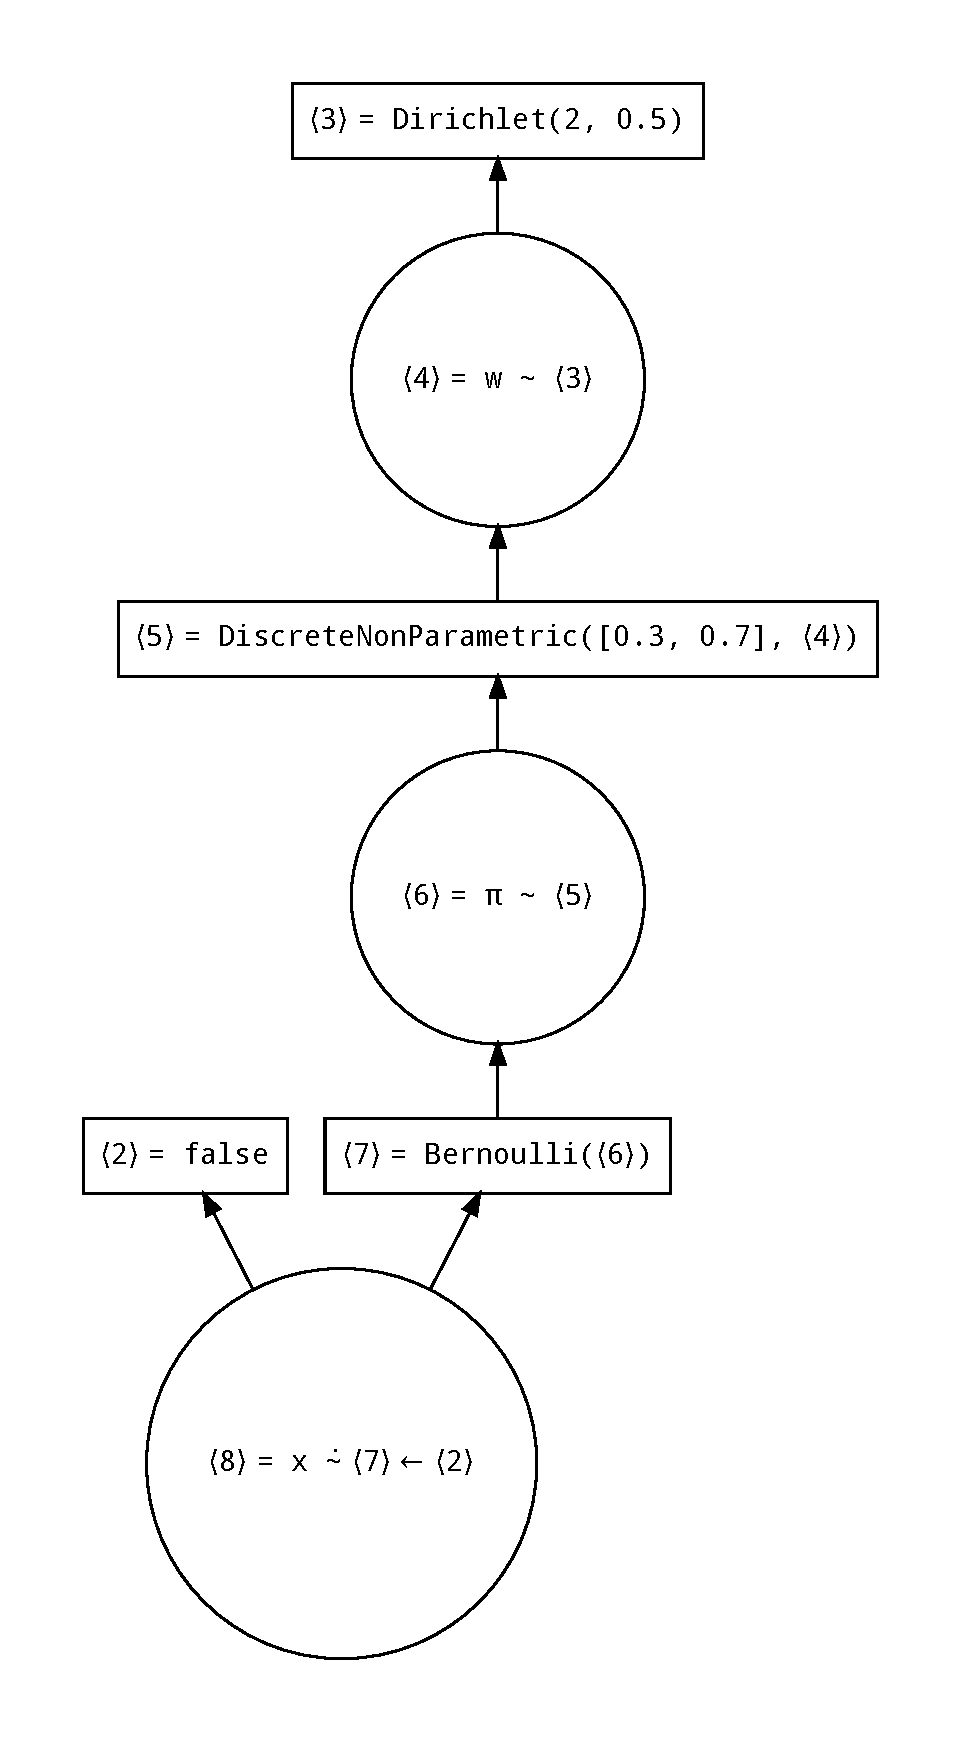
\includegraphics[width=0.49\textwidth]{figures/bernoulli_dependencies}}
  \subbottom[][\texttt{hierarchical\_gaussian(1.4)}]{%
    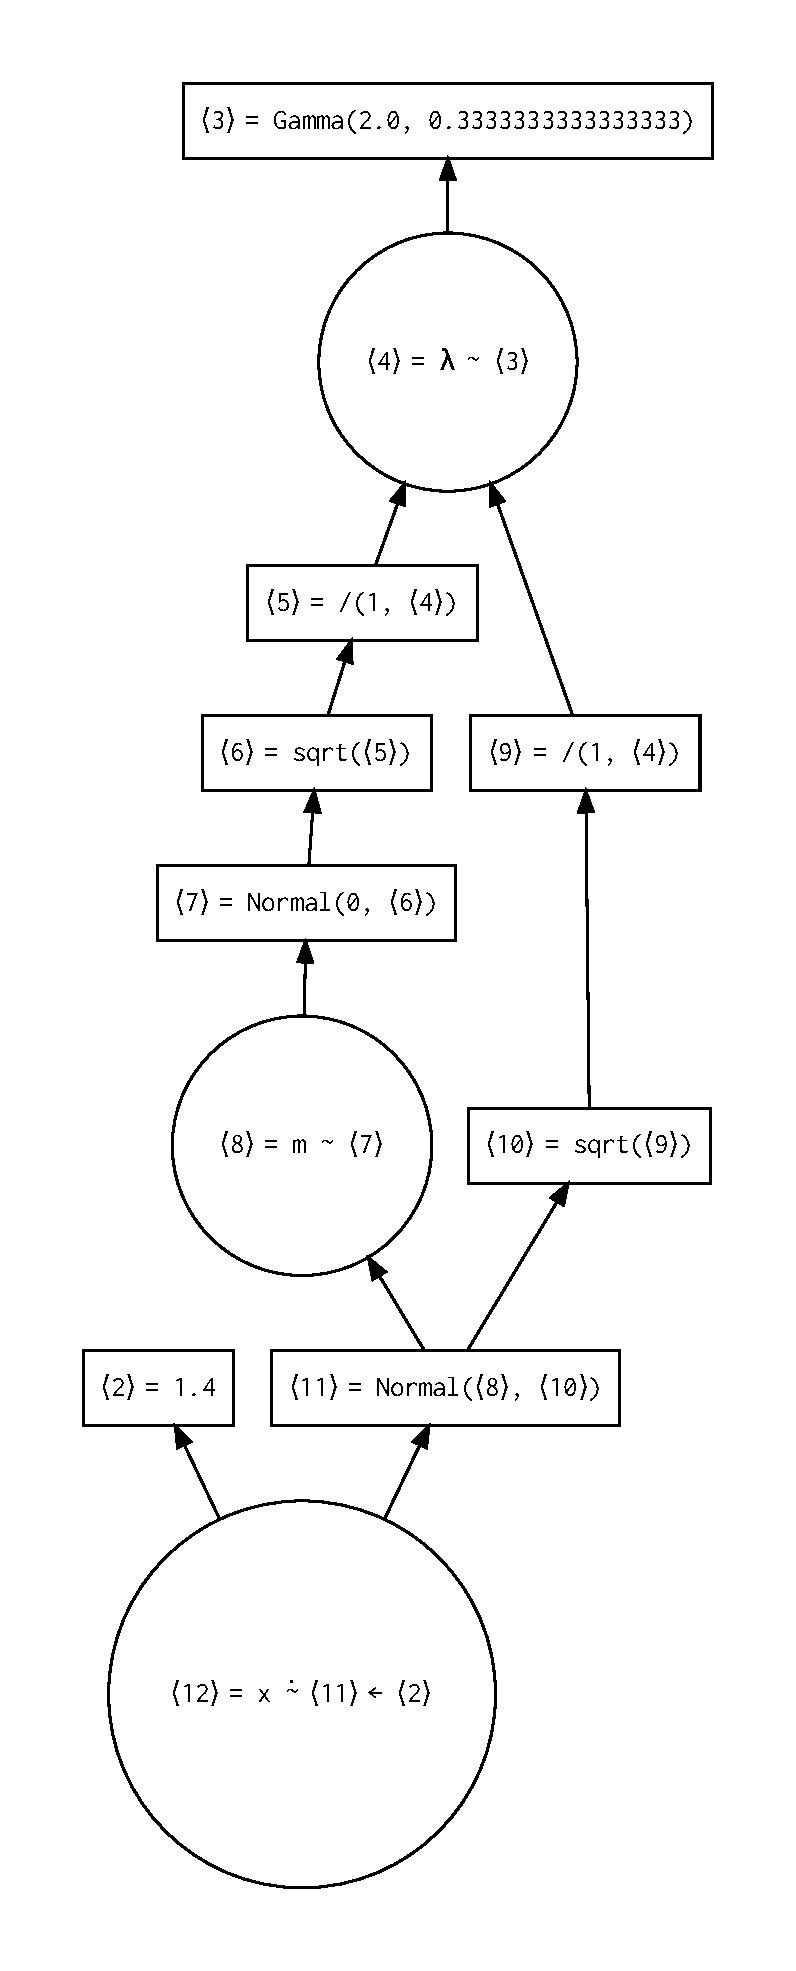
\includegraphics[width=0.49\textwidth]{figures/gaussian_dependencies}}
  \caption{Dependency graphs of the models in listing~\ref{lst:dependency-examples}, generated by
    \autogibbsjl{} and rendered by GraphViz.  More information, such as node values, is stored in
    the real model graph, but not printed for better readability.  Circular nodes denote tilde
    statements, while deterministic intermediate values, corresponding to normal SSA statements, are
    written in rectangles.}
  \label{fig:geom-deps}
\end{figure}


\section{Automatic Calculation of Gibbs Conditionals}
\label{sec:automatic-conditionals}

The ultimate contribution of this work is to utilize the dependency extraction system to extend
\turingjl{} with JAGS-style automatic calculation of Gibbs Conditionals.  In JAGS (and its sibling,
BUGS) conditional extraction works over a wide range of variable types \parencite{plummer2003jags}
by symbolic analysis and recognition of several patterns (e.g., conjugate distributions from
exponential families, log-concave or compactly supported distributions; see
\textcite{lunn2000winbugs}.), which is possible since the class of models is constrained by the
modeling language, and available in completely structured form.

In \turingjl{}, models are much less restricted, and the symbolic form has to recovered from
outside, as we have seen.  To focus on the principal ideas and not to extend the scope too much, the
implementation described in this section was restricted to finite, discrete conditionals, which are
trivial to sample from, given the respective log-density.  Since the construction of conditional
log-densities is independent from the normalization step, though, this can serve as a starting point
for further, more general conditional samplers, as those in JAGS and BUGS.  Additionally, and this
is a more fundamental limitation, the models to which the extraction algorithm can be applied must
be static in a specific sense: the whole Markov blanket of the variable in question must be unique,
and reachable within one run of model tracking.  A large fraction of the models used in practice
do fulfill this condition, though.  As this problem is difficult so solve in general, the same
constraint applies to JAGS and BUGS, which makes \autogibbsjl{} not more limited than these.

The implementation of the conditional extraction system involves three main steps:
\begin{enumerate}
  \firmlist
\item Extracting the symbolic form of the conditional likelihood of Markov blankets in a given
  dependency graph.
\item Constructing closures calculating the normalized discrete conditionals from these likelihoods.
\item Providing a Gibbs-component sampler for \turingjl{}, that can utilize the resulting
  conditional distributions.
\end{enumerate}
The third step turned out to be the easiest, since the sampling system of \turingjl{} is designed to
be extensible.  Ideally, a Gibbs-conditional sampler would have first been added to \turingjl{} and
then simply been reused for \autogibbsjl{}; in practice, it worked out the other way round, and the
\autogibbsjl{} sampler has, in generalized form, been added to \turingjl{} afterwards (without the
automatic extraction, only supporting user-provided conditional distributions).

\newsavebox{\bmlikelihoods}
\begin{lrbox}{\bmlikelihoods}
\begin{lstlisting}[style=lstfloat]
⟨2⟩ = 1.4                  ⤳ 1.4
⟨3⟩ = Dirichlet(2, 0.5)    ⤳ Dirichlet(2, 0.5)
⟨4⟩ = w ~ ⟨3⟩              ⤳ logpdf(Dirichlet(2, 0.5), θ[w])
⟨5⟩ = DNP([0.3, 0.7], ⟨4⟩) ⤳ DNP([0.3, 0.7], θ[w])
⟨6⟩ = π ~ ⟨5⟩              ⤳ logpdf(DNP([0.3, 0.7], θ[w]), θ[π])
⟨7⟩ = Bernoulli(⟨6⟩)       ⤳ Bernoulli(θ[p])
⟨8⟩ = x ~ ⟨7⟩ ← ⟨2⟩       ⤳ logpdf(Bernoulli(θ[p]), θ[x])
\end{lstlisting}
\end{lrbox}
\newsavebox{\hglikelihoods}
\begin{lrbox}{\hglikelihoods}
\begin{lstlisting}[style=lstfloat]
⟨2⟩ = 1.4                 ⤳ 1.4
⟨3⟩ = Gamma(2.0, 1/3)     ⤳ Gamma(2.0, 1/3)
⟨4⟩ = λ ~ ⟨3⟩             ⤳ logpdf(Gamma(2.0, 1/3), θ[λ])
⟨5⟩ = /(1, ⟨4⟩)           ⤳ /(1, θ[λ])
⟨6⟩ = sqrt(⟨5⟩)           ⤳ sqrt(/(1, θ[λ]))
⟨7⟩ = Normal(0, ⟨6⟩)      ⤳ Normal(0, sqrt(/(1, θ[λ])))
⟨8⟩ = m ~ ⟨7⟩             ⤳ logpdf(Normal(0, sqrt(/(1, θ[λ]))), θ[m])
⟨9⟩ = /(1, ⟨4⟩)           ⤳ /(1, θ[λ])
⟨10⟩ = sqrt(⟨9⟩)          ⤳ sqrt(/(1, θ[λ]))
⟨11⟩ = Normal(⟨8⟩, ⟨10⟩)  ⤳ Normal(θ[m], sqrt(/(1, θ[λ])))
⟨12⟩ = x ~ ⟨11⟩ ← ⟨2⟩    ⤳ logpdf(Normal(θ[m], sqrt(/(1, θ[λ]))), θ[x])
\end{lstlisting}
\end{lrbox}
\begin{figure}[t]
  \loosesubcaptions
  \subbottom[\texttt{bernoulli\_mixture(false)}]{\usebox{\bmlikelihoods}}
  \subbottom[\texttt{hierarchical\_gaussian(1.4)}]{\usebox{\hglikelihoods}}
  \caption{Association of the dependency graph of the example models from
    listing~\ref{lst:dependency-examples} with intermediate symbolic functions.  The expressions on
    the right are implicit functions of \protect\jlinl{θ}.  (\texttt{DNP} is used instead of
    \texttt{DiscreteNonParametric} to avoid breaking lines.)}
  \label{fig:continuations}
\end{figure}

Step 1, the symbolic extraction of likelihood functions, is implemented by first converting the full
trace into a symbolic joint log-density.  Therefor the expression of each node in the dependency
graph is associated with a corresponding symbolic representation of a function of the \enquote{trace
  dictionary} \jlinl{θ}, which holds the values of the random variables by name (this is to view the
probabilistic model as a joint distribution over trace dictionaries).  This is done in the following
simple fashion:
\begin{itemize}
  \firmlist
\item References to call nodes or constant nodes (\jlinl{⟨i⟩ = x}) are inlined.
\item References to tilde nodes (\jlinl{⟨j⟩ = v ~ D}) are converted to dictionary lookups: \jlinl{θ[v]}.
\item Call nodes are converted to functions from the trace dictionary to a
  function call on the converted references: \jlinl{f(⟨i⟩, ⟨j⟩)} \(\leadsto\) \jlinl{f(x, θ[v])}.
\item Tilde nodes are converted to log-density evaluations of their values given the corresponding
  distribution: \jlinl{⟨j⟩ = v ~ D} \(\leadsto\) \jlinl{logpdf(D, θ[v])}
\end{itemize}
All resulting expressions are thereby to be understood as implicit functions of \jlinl{θ}.  These
new expression function objects can then be numerically evaluated as log-densities for given values
of all random variables.  For illustration, the joint densities of the \jlinl{bernoulli_mixture} and
\jlinl{hierarchical_gaussian} models introduced above in listing~\ref{lst:dependency-examples}, are
associated with corresponding symbolic functions as shown in figure~\ref{fig:continuations}\todo{fix
  caption alignment}.  By adding the log-likelihoods for each tilde statement, we get the symbolic
log-joint density as, for example,
\begin{lstlisting}
logpdf(Gamma(2.0, 0.333333), θ[λ]) + 
  logpdf(Normal(0, sqrt(/(1, θ[λ]))), θ[m]) + 
  logpdf(Normal(θ[m], sqrt(/(1, θ[λ]))), θ[x]),
\end{lstlisting}
corresponding to the density over \(\lambda\), \(m\), and \(x\), factorized as
\begin{equation}
  p(\lambda, m, x) = p(\lambda) \, p(m \given \lambda) \, p(x \given m, \lambda).
\end{equation}
From this we can then derive conditionals in the usual way of normalizing the proportional
conditional, which can be obtained by removing all terms of the joint factorization that do not
depend on the conditioned variable:
\begin{equation}
  \begin{aligned}
    p(m \given \lambda, x) &\propto p(m \given \lambda) \, p(x \given m, \lambda), \\
    p(\lambda \given m, x) &\propto p(\lambda) \, p(m \given \lambda) \, p(x \given m, \lambda),
  \end{aligned}
\end{equation}
which in more technical terms are given through the \emph{Markov blanket} of \(m\) and \(\lambda\)
\parencites[section 24.2]{murphy2012machine}[section 4.5]{koller2009probabilistic}.

The crucial problem here is, of course, to find the normalization factor, as always in Monte Carlo
methods.  Normalization could, for example, be implemented by analysing the structure of the
resulting expression and detecting conjugacies, such as the normal/normal-gamma relationship between
\(m\), \(\lambda\), and \(x\) above.  The simplest possible case, however, occurs when when a
conditioned variable has finite support; and as mentioned above, this is what has been implemented
out in this work.  For example, \(p\) in the \jlinl{bernoulli_mixture} model is such a finitely
supported variable~-- we get
\begin{equation}
    p(\pi \given w, x) = \frac{p(w) \, p(\pi \given w) \, p(x \given \pi)}{
      \sum_{\varpi \in \{0.3, 0.7\}}p(w) \, p(\varpi \given w) \, p(x \given \varpi)}
\end{equation}
Since the distribution of every variables is preserved in the dependency graph, we now can do the
same thing programmatically, and turn the symbolic log-density into a distribution object by simply
tabulating the values of the denominator through evaluating of the expression over the whole support
of \(\pi\), the set \(\{0.3, 0.7\}\), and summing it up to get the normalization factor.  (This uses
the interface of distribution objects from the \juliapackage{Distributions.jl} package, which have a
\jlinl{support} method whose result is an iterable.)

Concretely, the construction works as follows, finalizing step 2 of the above scheme, exemplified by
\jlinl{bernoulli_mixture}:
\begin{enumerate}
  \firmlist
\item Find the likelihood expressions that match a given conditioned variable (this includes indexed
  variables subsumed by a parent, like \jlinl{v[i]} and \jlinl{v}), and their distribution:
  \begin{equation*}
    \begin{aligned}
      \ell_{1} &= \mathtt{logpdf(DNP([0.3, 0.7],\theta[w]), \theta[\pi])}. \\
      \mathcal{D} &= \mathtt{DNP([0.3, 0.7], \theta[w])}.
    \end{aligned}
  \end{equation*}
\item For each of these (sub-)variables, collect the likelihoods of their children variables, thus
  completing the Markov blanket:
  \begin{equation*}
    \ell_{2} = \mathtt{logpdf(Bernoulli(\theta[\pi]), \theta[x])}
  \end{equation*}
  The complicated part of this and the previous step is the correct matching of indexed variables in
  the trace dictionary: forms like \jlinl{θ[v][1]} and \jlinl{θ[v[1]]} need to be resolved correctly
  to the same value.
\item Construct for each a closure function that takes as an argument a fixed trace dictionary,
  tabulates the conditional log-likelihood over it with the conditioned variable fixed to all values
  of its support, and normalizes the result:\todo{Better typesetting?}
  \begin{equation*}
    \begin{aligned}
      &\theta \mapsto \{ \\
      &\quad \Omega = \mathtt{support}(\mathcal{D}) \\
      &\quad \mathtt{table} = \left[\operatorname{eval}(\ell_{1}, \theta[\pi \leadsto \varpi]) +
        \operatorname{eval}(\ell_{2}, \theta[\pi \leadsto \varpi]) \mid \varpi \in \Omega \right] \\
      &\quad \distr{DNP}(\Omega, \operatorname{softmax}(\mathtt{table})) \\
      &\}
    \end{aligned}
  \end{equation*}
  (whereby \(\operatorname{softmax}(x) = \broadcast{\exp}(x) / \sum_i \exp(x_{i})\) is the
  normalization operation on log-probabilities).
\end{enumerate}
The result of this process is a collection of closures that represent the conditional likelihoods as
\enquote{kernels}: functions from conditioned-on variables to distribution objects.  These closures
can then be used to construct a conditional sampler for usage in \turingjl{}'s \jlinl{Gibbs}
sampler, in combination with other samplers for the continuous variables.

\newthought{As for potential improvements}, there is of course a wide range of possibilities, as the
current implementation is a most primitive one.  As has been mentioned before, further classes of
random variables beyond those with finite support could be handled, using methods and heuristics as
in BUGS or JAGS.  This could even involve symbolic methods like those in AutoConj
\parencite{hoffman2018autoconj}. More generally, variance-reducing transformation, as those in
\textcite{murray2017delayed}, are applicable.  For computational efficiency, a parallel Gibbs
sampler \parencite{gonzalez2011parallel} could be constructed, improving scalability with increasing
data size (i.e., numbers of observations).  Or, as in \juliapackage{Gen.jl}, a variant of
\enquote{argument diffs} could be devised to prevent unnecessary re-evaluation of model parts
\parencites[see][section 1.2.3]{cusumano-towner2020gen}{becker2020dynamic}.

Besides improvements via inference algorithms, it would be possible for models that are written in a
vectorized or otherwise \enquote{trace constant} fashion, such that the structure of the
conditionals does not change with the number of observations, to record the trace for a small model
and reuse it for arbitrary larger ones, thus avoiding recomputation and recompilation.  Finally, the
evaluation of the conditional closures, which is currently performed by simple interpretation of
expressions, could be sped up by compiling them to Julia methods, or even better by reusing the
SSA-like structure to emit Julia IR directly.

Realistically, though, I consider it more worthwhile to follow a different approach, like the one
outlined in section~\ref{sec:future-work} below, and moving away from working on a trace-based
reconstruction and to a domain-specific intermediate representation with generalized transformation
capabilities.  On such a representation, all of the named ideas still apply, but it would have the
advantage of being more invariant to a specific inference system, and be able to handle more general
probabilistic programs (foremost, not only static ones).


\section{Evaluation}
\label{sec:autogibbs-eval}

To begin with a qualitative assessment, it must be admitted that \autogibbsjl{} is, when run
manually and only once, empirically so noticeably slow, that a user may be tempted to dismiss it
outright (concretely speaking, extraction of one conditional for some not-so-large models takes
\(20\) to \(200\) seconds on the author's laptop).  This is a valid point, but two counter-arguments
must be considered.  For one, the implementation is a preliminary one, more conceptual than
optimized.  Much of the slow-down could be mitigated by just improving key parts of \autogibbsjl{}
and \irtrackerjl{}.

In addition to that, one must realize where this apparent slowness comes from: namely, from
compilation, and therein primarily type inference, of the functions handling all the strongly typed
expression trees.  Besides the possibility of just optimizing these further, the following fact is
most important to realize: compilation takes place only once~-- as soon as a conditional is
constructed, it can be reused in arbitrarily many sampling runs of the same model.  The finished
conditionals then do not take so much time anymore, quite the contrary: they are much faster than
other within-Gibbs samplers, since they only involve evaluating a fixed expression, constructing a
distribution, and sampling from it once (and even this could be sped up further).  This makes it
possible to sample much longer chains in the same time, which is an overall advantage.

Furthermore, due to the limitations \autogibbsjl{} puts on the structure of variable names, there
are cases in which models cannot be formulated in a certain desirable way in \dppljl{}, thus losing
certain advantages such as block-wise treatment of collections of independent variables.  This can
lead to a disadvantage compared to other samplers.  Again, the restrictions are mostly a detail of
the current implementation, and there is no theoretical hindrance in overcoming than.

So, to conclude, while the implementation in current form is not applicable in practice for all
possible cases, it is very much so in principle.  Based on the lessons learned through this work,
further contributions to Gibbs sampling in \turingjl{} are already planned (although not necessarily
based on \autogibbsjl{}).

\newthought{For a more {q}uantitative} point of view, let us now turn to some empirical evaluations.
Besides several unit tests for correctness of the derived dependencies and conditionals on a variety
of small models chosen to test certain features and corner cases, an experimental comparison of
\autogibbsjl{} and existing \turingjl{} samplers has been conducted.  Three off-the-shelf Bayesian
models were chosen: a Gaussian mixture model (GMM) with known variances and priors over cluster
centers, weights, and assignments \parencite[section 6.2]{marin2007bayesian}:
\begin{equation}
  \label{eq:gmm}
  \begin{aligned}
    w &\from \distr{Dirichlet(K)} \\
    z_{n} &\from \distr{Categorical}([1, \ldots, K], w), \quad n = 1, \ldots, N \\
    \mu_{k} &\from \Normal(0, \sigma_{1}), \quad k = 1, \ldots, K \\
    x_{n} &\from \Normal(\mu_{z_{n}}, \sigma_{1}), \quad n = 1, \ldots, N;
  \end{aligned}
\end{equation}
a hidden Markov model
(HMM) with known variances and priors over transition and emission probabilities \parencite[section
7.3]{marin2007bayesian}:
\begin{equation}
  \label{eq:hmm}
  \begin{aligned}
    T_{k} &\from \distr{Dirichlet}(K), \quad k = 1, \ldots, K \\
    m_{k} &\from \Normal(k, \sigma_{1}), \quad k = 1, \ldots, K \\
    s_{1} &\from \distr{Categorical}([1, \ldots, K], [1/K, \ldots, 1/K]) \\
    s_{k} &\from \distr{Categorical}([1, \ldots, K], T_{s_{k-1}}), \quad k = 2, \ldots, N \\
    x_{k} &\from \Normal(m_{s_{k}}, \sigma_{2}), \quad k = 1, \ldots, N;
  \end{aligned}
\end{equation}
and an infinite mixture model (IMM) in stick-breaking construction, but
otherwise of the same form as the GMM, to represent a nonparametric example \parencite[section
2.2]{hjort2010bayesian}:
\begin{equation}
  \label{eq:imm}
  \begin{aligned}
    w &\from \distr{TruncatedStickBreakingProcess(\alpha, K)} \\
    z_{n} &\from \distr{Categorical}([1, \ldots, K], w), \quad n = 1, \ldots, N \\
    \mu_{k} &\from \Normal(0, \sigma_{1}), \quad k = 1, \ldots, K \\
    y_{n} &\from \Normal(\mu_{z_{n}}, \sigma_{2}), \quad n = 1, \ldots, N.
  \end{aligned}
\end{equation}
In the context of this work, the three interesting classes of metrics are
\begin{enumerate}
  \firmlist
\item the \enquote{extraction time} of \autogibbsjl{}, i.e., the time it takes to extract and a
  conditional including compilation times,
\item the sampling speed when used as component of a within-Gibbs sampler, and
\item the quality of the resulting chains, in terms of convergence and variance diagnostics.
  (Although this really measures Gibbs sampling, not the implementation of \autogibbsjl{}, it is a
  relevant comparison for the practitioner.)
\end{enumerate}
To estimate them, a series of experiments has been conducted.  Each of the test models involves one
discrete and two continuous parameter arrays.  As a baseline for \autogibbsjl{}'s static conditional
(AG), \turingjl{}'s Particle Gibbs sampler (PG) was chosen, which is also suited to discrete
parameters.  PG was always used with \(100\) particles, since lower values did not lead to
convergent chains.  Continuous variables were all sampled using Hamiltonian Monte Carlo (HMC) with
hand-tuned parameters (\(10\) leapfrog steps with step size \(0.05\)).  The experiments have been
set up to vary between AG and PG, and between \(10\), \(25\), and \(50\) observations, since their
number determines the size of the trace, and thus influences both AG's compile times and the overall
sampling time.  All measurements were conducted using the following system configuration, as shown
by \jlinl{InteractiveUtils.versioninfo()}:
\begin{lstlisting}
Julia Version 1.3.1
Commit 2d5741174c (2019-12-30 21:36 UTC)
Platform Info:
  OS: Linux (x86_64-pc-linux-gnu)
  CPU: Intel(R) Core(TM) i5-4690 CPU @ 3.50GHz
  WORD_SIZE: 64
  LIBM: libopenlibm
  LLVM: libLLVM-6.0.1 (ORCJIT, haswell)
\end{lstlisting}
Everything was executed single-threaded, with exclusive resource access on the server, to preclude
measurement noise as much as possible.  Each of the three models was benchmarked in a separate Julia
session.  The last two chains of the HMM with \(50\) observations using Particle Gibbs could not be
completed, due to the twelve hour time limit set by the job scheduler.  The raw data can be found in
\textcite{gabler2020mcmc}. 

The \dppljl{} implementations of the models can be found in listing~\ref{lst:evaluation-models}.
Note that for each, there exists a second, equivalent implementation used for PG, since particle
samplers in \turingjl{} require the usage of special data types due to their task copying mechanism.

\newthought{It follows} a detailed analysis of the results per model in graphical form, based on six
plots each.  First, PG and AG are compared in terms of sampling times by number of observations on
the top left.  Right of this, we have the dependency of the extraction time of AG given the number
observations.  The first of these points is almost always an outlier, since it involves additional
compilation time.  Through the rest, a quadratic function is fitted, which always matched the values
very closely.

On the recto pages, plots for convergence analysis are visualized.  Since these are estimated per
parameter, and the test models involve larger arrays of parameters, the first elements of the
continuous and the fifth element of the discrete parameters have always been chosen as
representatives.  On the top, the first chain of each experimental combination is shown as a
qualitative representative (thinned for ease of plotting).  Well-converging chains should look like
white noise, not like a random walk.  In the middle plot, the estimated autocorrelation functions of
the same chains are given, which are a way to evaluate convergence speed by eye.  The functions
should vanish quickly (indicated by the gray significance bar around the abscissa); uncorrelated
samples would have zero autocorrelation except for the first lag.

Lastly, two diagnostic values are plotted for each combination and chain.  The
\enquote{scale-reduction} \(\widehat{\mathrm{R}}\), after \textcite{gelman1992inference}, estimates
the factor by which the scale of the current distribution might be reduced if the simulations were
continued \parencite[see][p. 285]{gelman2020bayesian}.  It should be close to one for indicating
good convergence; as a rule of thumb, a value of more than \(1.1\) is suspicious.  The effective
sample size (ESS) arises in the estimation of the asymptotic variance of Markov chains
\parencite[][section 7.2]{vihola2020lectures}, where it is formally analogous to the sample size in
the variance estimator for \iid{} variables.  The ESS can also be interpreted as a one-point summary
of the autocorrelation estimate, normalized by chain length.  It should be close to the actual
number of samples, or at least of the same order of magnitude.

%%%%%%%%%%%%%%%%%%%%%%%%%%%%%%%%%%%%%%%%%%%%%%%%%%%%%%%%%%%%%%%%%%

\begin{lstfloat}[p]
\begin{lstlisting}[style=lstfloat]
@model function gmm(x, K)
    N = length(x)
    w ~ Dirichlet(K, 1/K)  # Cluster association prior
    z ~ filldist(Categorical(w), N)  # Cluster assignments
    μ ~ filldist(Normal(0.0, s1_gmm), K)  # Cluster centers

    for n = 1:N
        x[n] ~ Normal(μ[z[n]], s2_gmm)  # Observations
    end
end

@model function hmm(x, K, ::Type{T}=Float64) where {T<:Real}
    N = length(x)

    T = Vector{Vector{X}}(undef, K)
    for i = 1:K
        T[i] ~ Dirichlet(K, 1/K)  # Transition probabilities
    end
    
    s = zeros(Int, N)
    s[1] ~ Categorical(K)
    for i = 2:N
        s[i] ~ Categorical(T[s[i-1]])  # State sequence
    end
    
    m = Vector{T}(undef, K)
    for i = 1:K
        m[i] ~ Normal(i, s1_hmm)  # Emission probabilities
    end
    
    x[1] ~ Normal(m[s[1]], s2_hmm)
    for i = 2:N
        x[i] ~ Normal(m[s[i]], s2_hmm)  # Observations
    end
end

@model function imm_stick(y, α, K)
    N = length(y)
    crm = DirichletProcess(α)
    v ~ filldist(StickBreakingProcess(crm), K - 1)
    w = stickbreak(v)  # Cluster weights
    
    z = zeros(Int, N)
    for n = 1:N
        z[n] ~ Categorical(w)  # Cluster assignments
    end

    μ ~ filldist(Normal(0.0, s1_imm), K)  # Cluster centers

    for n = 1:N
        y[n] ~ Normal(μ[z[n]], s2_imm)  # Observations
    end
end
\end{lstlisting}
  \caption{Gaussian mixture model, hidden Markov model, and infinite mixture model using a
    stick-breaking construction.  The two-step calculation of \texttt{w} via \texttt{v} is a
    technicality due to \turingjl{}'s handling of nonparametric models.  The function
    \texttt{stickbreak} normalizes the stick-lengths \texttt{v} into a Dirichlet-like distribution.
    The \texttt{Categorical(p)} constructor automatically infers the support of the categorical
    distribution from the weight vector as \texttt{1:length(p)}.}
  \label{lst:evaluation-models}
\end{lstfloat}

%%%%%%%%%%%%%%%%%%%%%%%%%%%%%%%%%%%%%%%%%%%%%%%%%%%%%%%%%%%%%%%%%%
\cleartoverso
\FloatBlock

\newcommand{\leftplotcaption}[1]{%
  Sampling and extraction times for #1, factored by algorithm and number
  of observations.  Points are jittered horizontally to increase readability.  A quadratic curve is
  fitted to the extraction times.
}
\newcommand{\rightplotcaption}[1]{%
  Diagnostics, factored by algorithm, number of observations, and a selection of model parameters.
  \(\widehat{\mathrm{R}}\) and ESS point estimates are jittered horizontally for better readability.
  For chain plots and autocorrelation, the first chain of the respective combination has been used.
}

\begin{figure}[t!]
  \centering
  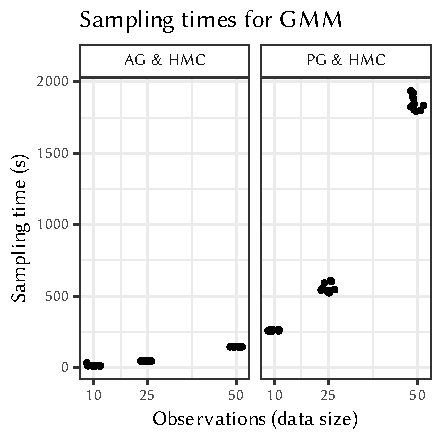
\includegraphics[width=0.49\textwidth]{figures/GMM-sampling_times}
  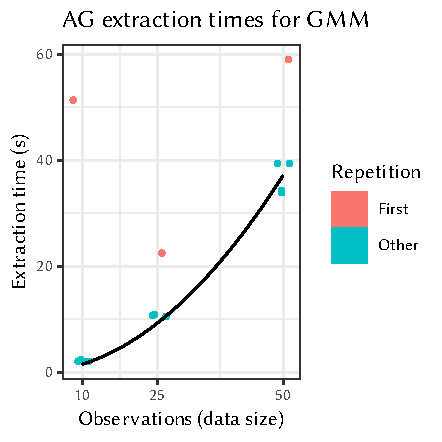
\includegraphics[width=0.49\textwidth]{figures/GMM-compile_times}
  \caption{\leftplotcaption{GMM}}
  \label{fig:plots-gmm}
\end{figure}

\subsection*{Gaussian Mixture Model}

For the GMM, the AG sampling times lie consistenly below the minimum of the PG sampling times, even
with the largest number of observations.  Extraction time seems to grow quadratically, with
exception of the first call of the conditional extraction, involving compilation and type
inference.

The mixing behaviour of the chains shows a large variation.  With \(10\) and \(25\) observations,
neither of the altgorithms reaches consistently satisfactory results; the distribution of
\(\widehat{R}\) values is quite diffuse and suspiciously large (more so for PG), and especially the
ESS numbers are way too low.  A look at the exemplary autocorrelation plots seems to confirm bad
convergence.  The corresponding chains clearly show random-walk-like or \enquote{lumped} behaviour
for some combinations.

For \(50\) observations, the result is different with AG.  The \(w\) and \(\mu\) parameters appear
to converge well in most cases, with very low-variance chains and visibly large ESS values.  But for
unknown reasons, the \(z\) parameter seems to have gotten \enquote{stuck} in this particular example
and not moved at all, which is the reason no autocorrelation function could be estimated.  PG might
have improved somewhat, looking at the lower \(\widehat{R}\) distributions, but not enough to make a
meaningful difference, as ESS and autocorrelation plots show no sufficiently good behaviour.


\cleartorecto
\FloatBlock

\begin{figure}[p]
  \centering
  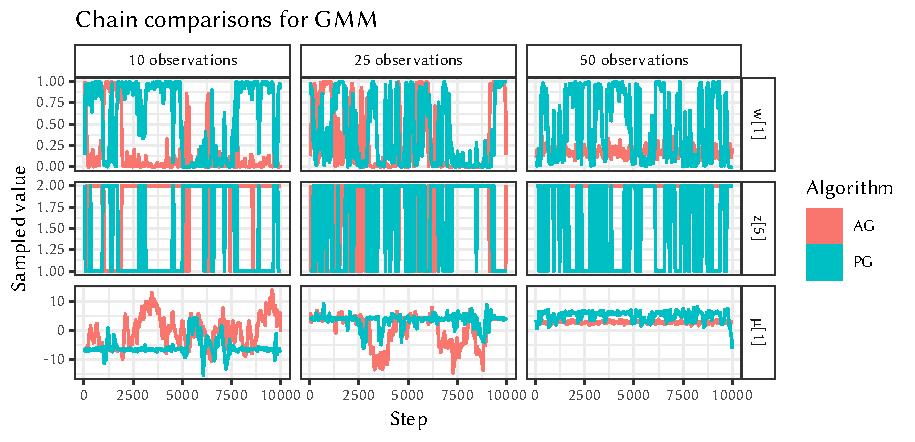
\includegraphics[width=\textwidth]{figures/GMM-chains}
  \par
  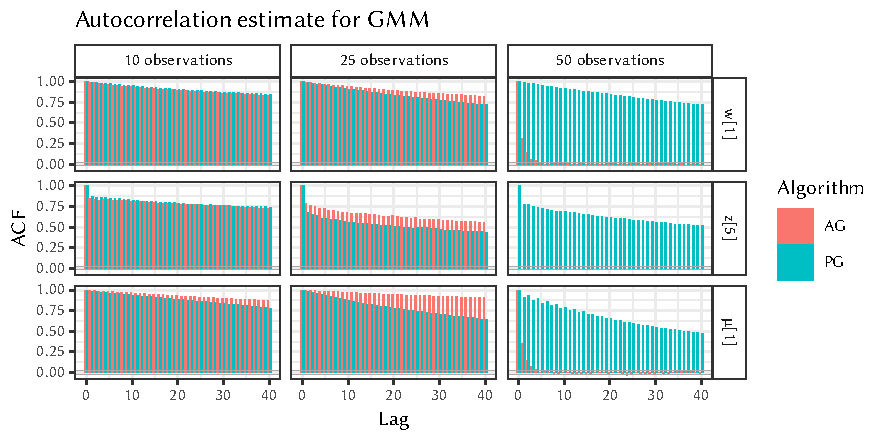
\includegraphics[width=\textwidth]{figures/GMM-acfs}
  \par
  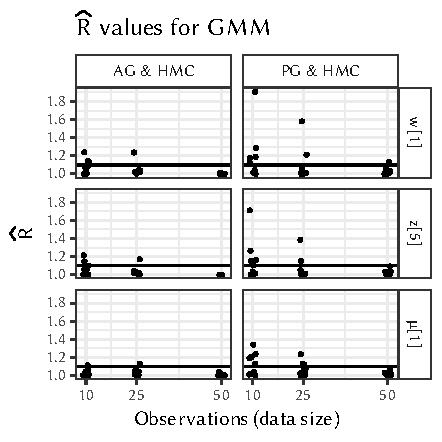
\includegraphics[width=0.49\textwidth]{figures/GMM-rhat}
  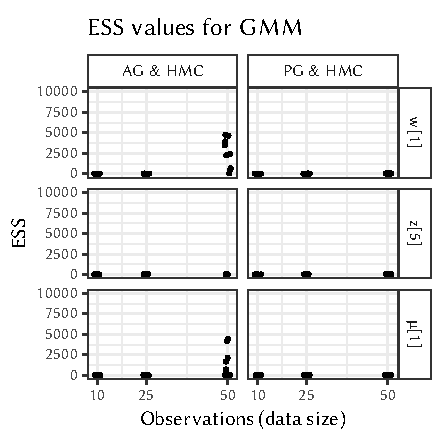
\includegraphics[width=0.49\textwidth]{figures/GMM-ess}
  \contcaption{\rightplotcaption{GMM}}
\end{figure}

%%%%%%%%%%%%%%%%%%%%%%%%%%%%%%%%%%%%%%%%%%%%%%%%%%%%%%%%%%%%%%%%%%
\cleartoverso
\FloatBlock

\begin{figure}[t!]
  \centering
    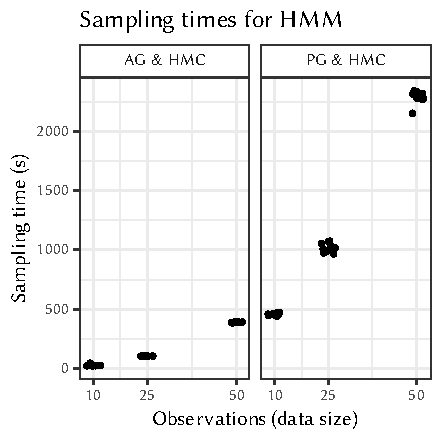
\includegraphics[width=0.49\textwidth]{figures/HMM-sampling_times}
  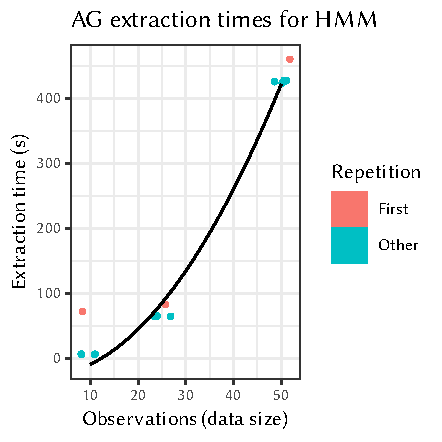
\includegraphics[width=0.49\textwidth]{figures/HMM-compile_times}
  \caption{\leftplotcaption{HMM}}
  \label{fig:plots-hmm}
\end{figure}

\subsection*{Hidden Markov Model}

Also for HMM, the same trends in sampling and extraction times as with GMM are visible, with AG
being consistenly faster.  The extraction times seem to be quite the same as GMM, even in absolute
terms, as are the outliers of the first function calls.

Mixing behaviour for this model is much better overall.  The chains look less like random walks,
especially for \(\mu\).  Autocorrelation plots are sometimes quite good, especially for \(s\), and
in all cases better as those above for GMM.  The \(\widehat{R}\) values are all in better ranges
(note the difference in the scale of the ordinate!), and ESS noticeably higher.  Overall, AG seems
to improve over PG on average, although neither of the results is stellar.

\cleartorecto
\FloatBlock

\begin{figure}[p]
  \centering
  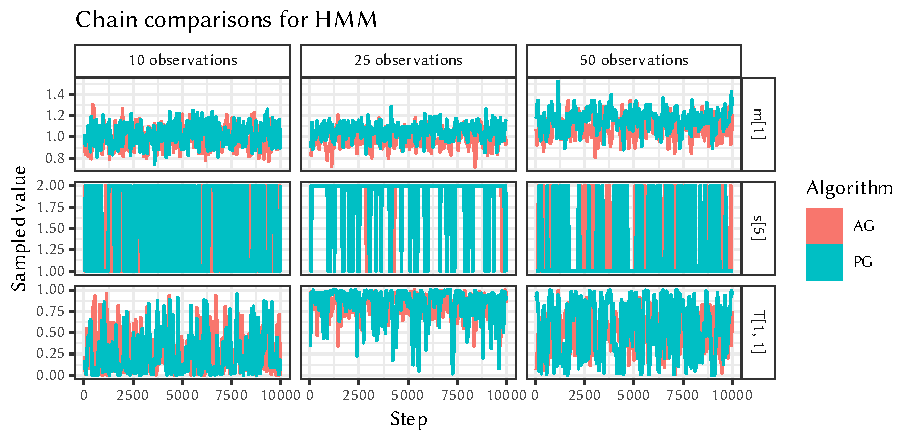
\includegraphics[width=\textwidth]{figures/HMM-chains}
  \par
  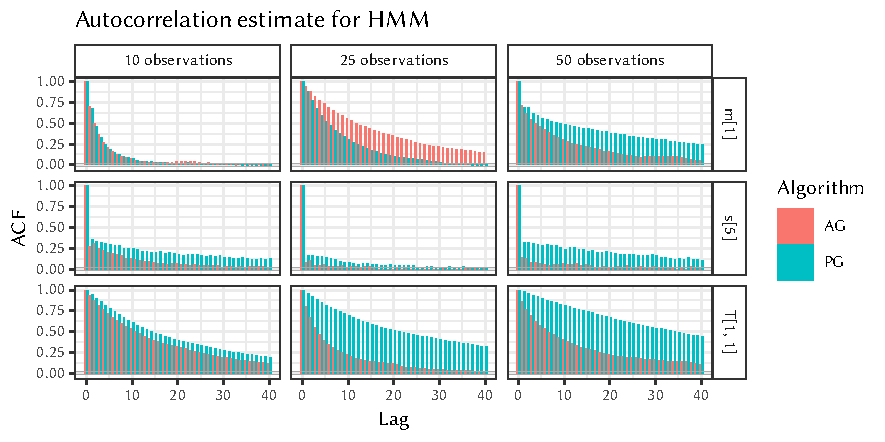
\includegraphics[width=\textwidth]{figures/HMM-acfs}
  \par
  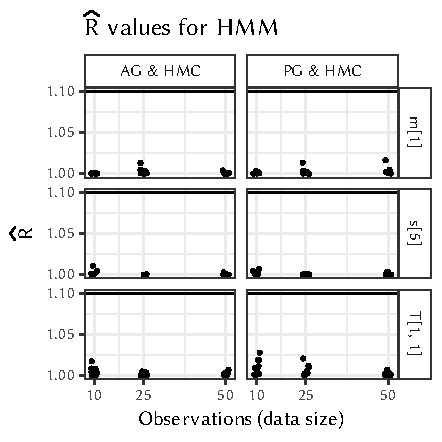
\includegraphics[width=0.49\textwidth]{figures/HMM-rhat}
  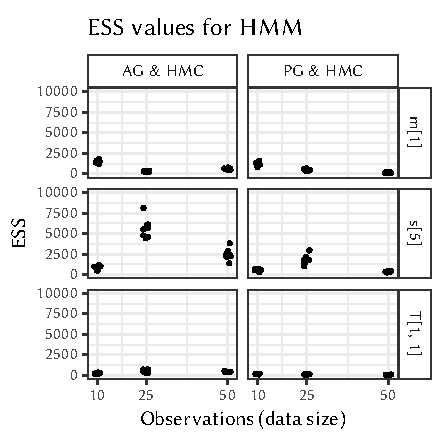
\includegraphics[width=0.49\textwidth]{figures/HMM-ess}
  \contcaption{\rightplotcaption{HMM}}
\end{figure}

%%%%%%%%%%%%%%%%%%%%%%%%%%%%%%%%%%%%%%%%%%%%%%%%%%%%%%%%%%%%%%%%%%
\cleartoverso
\FloatBlock

\begin{figure}[t!]
  \centering
  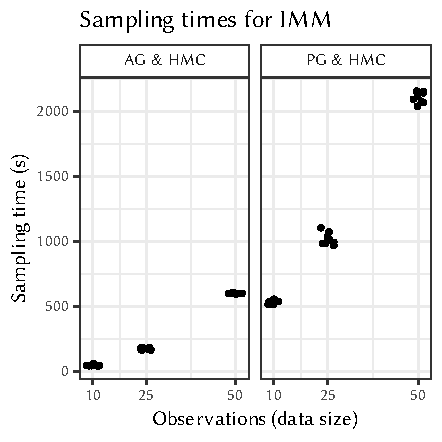
\includegraphics[width=0.49\textwidth]{figures/IMM-sampling_times}
  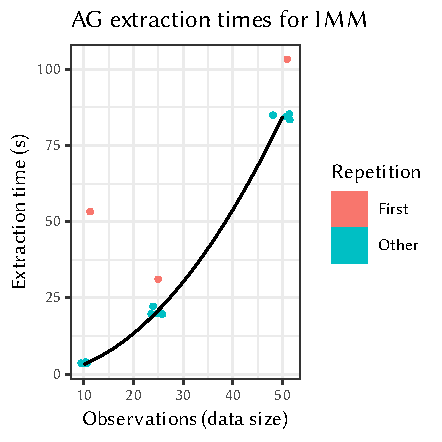
\includegraphics[width=0.49\textwidth]{figures/IMM-compile_times}
  \caption{\leftplotcaption{IMM}}
  \label{fig:plots-imm}
\end{figure}

\subsection*{Infinite Mixture Model}

Again, similar trends of sampling times and extraction times are noticeable.  Here we can observe
some larger involved factors, though; both curves grow faster, with PG on \(10\) observations even
being faster than AG on \(50\) observations; although still on a significantly higher scale in
general.

In this example, PG appears to work better on average.  In the example chain plots, we can only see
a noticeable difference for \(\mu\), while the autocorrelation graphs are almost all worse for AG
(although both algorithms seem to do better than in the GMM test).  ESS is only satisfactory for the
\(z\) parameters, but PG here shows a much more consistent behaviour of the \(\widehat{R}\)
distribution.


\begin{figure}[p]
  \centering
  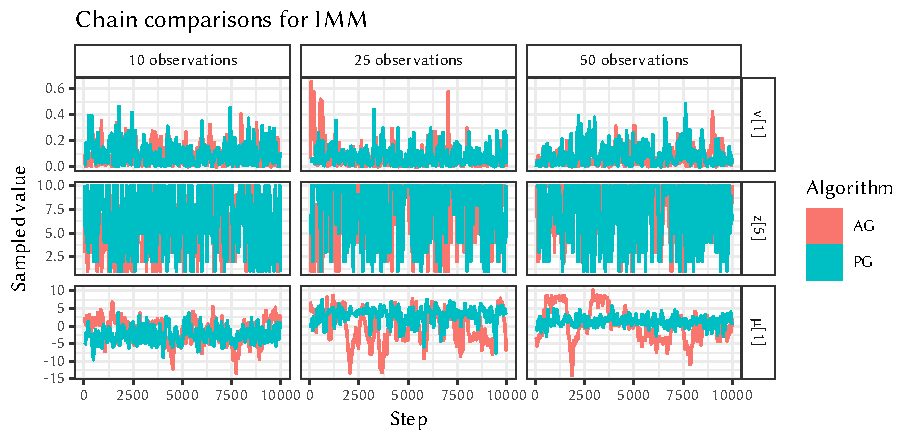
\includegraphics[width=\textwidth]{figures/IMM-chains}
  \par
  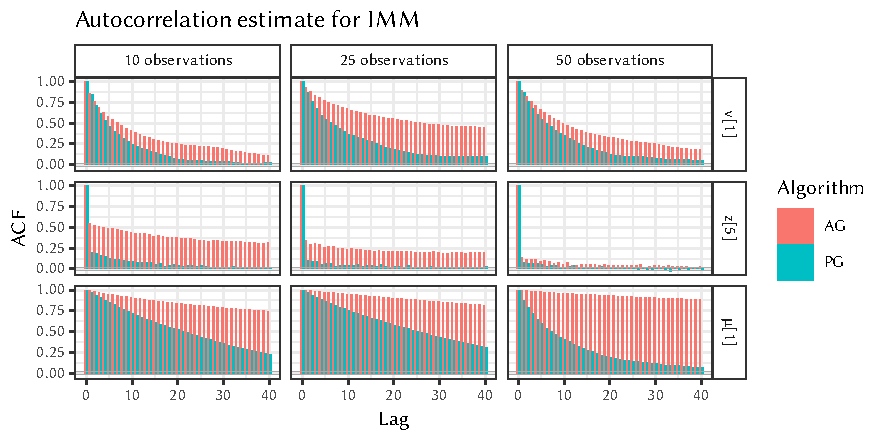
\includegraphics[width=\textwidth]{figures/IMM-acfs}
  \par
  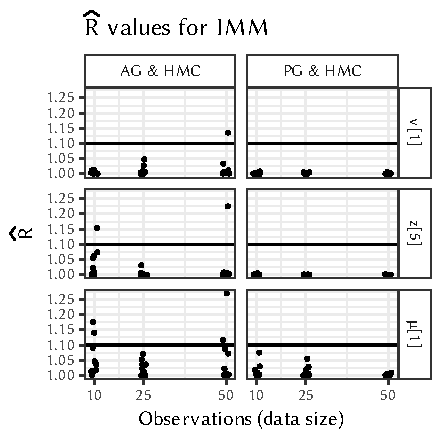
\includegraphics[width=0.49\textwidth]{figures/IMM-rhat}
  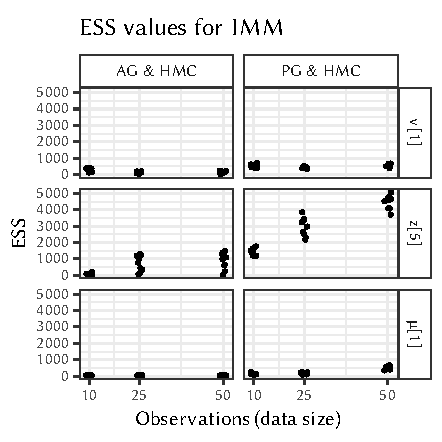
\includegraphics[width=0.49\textwidth]{figures/IMM-ess}
  \contcaption{\rightplotcaption{IMM}}
\end{figure}

\FloatBlock


\subsection*{Summary}

Whereas the sampling times of Particle Gibbs always grows rather fast, depending on the number of
observations, the rate of growth seems to be much lower for AutoGibbs.  The behaviour of these
curves appears to be superlinear, perhaps quadratic.  For GMM and HMM, the maximal sampling time of
AG is always below the minimal sampling time of PG.  Even in the case of IMM, AG's sampling time
with \(50\) observations is closest to PG's with only \(10\) particles, with the latter still
obviously rising much faster.

With regard to the extraction times, we can note a pretty clear quadratic run time depending on the
number of observations.  The first run is always significantly above this trend, due to the impact
of compilation and type inference.  Additionally, the first invocation for the lowest number of
observations might have involved additional compilation of library functions, explaining the larger
residual compared to the first runs of the larger numbers.

In terms of convergence, AG and PG deliver quite comparable results, varying with some variation in
quality depending on model and number of observations.  In most cases, judging by eye through the
exemplary autocorrelation plots, one or the other seems to slightly beat the other, which is
buttressed by the distribution of the diagnostic values.  IMM seems poses a particularly bad
application for AG, but otherwise, no consistent \enquote{winner} is visible, and variations do not
seem to follow a consistent pattern.

In conclusion, it can be said that for models where both are applicable, AutoGibbs provides a viable
alternative to PG, delivering comparable results in less time.  Care has to be taken to diagnose
mixing behaviour, though, as always in MCMC simulations.


% \begin{table}[t]
%   \centering
%   \libertineTabular
%   \begin{tabularx}{\textwidth}{XXrrr@{\hskip 10mm}rrrr}
%     \toprule
%      & & \multicolumn{3}{c@{\hskip 10mm}}{\textbf{GMM}} & \multicolumn{3}{c}{\textbf{HMM}} & \multicolumn{1}{c}{\textbf{IMM}} \\
%     \midrule
%     & HMC Step size & & 0.05 & & & 0.05 & & 0.05 \\
%     & HMC Steps & & 10 & & & 10 & & 10 \\
%     \midrule
%     \textbf{AG + HMC} & Observations & 10 & 25 & 50 & 10 & 25 & 50 & 10 \\
%     & Chains & 30 & 30 & 30 & 30 & 30 & 30 & 30 \\
%     & Compilations & 3 & 3 & 3 & 3 & 3 & 3 & 3 \\
%     \addlinespace
%     \textbf{PG + HMC,} & Observations & 10 & 25 & 50 & 10 & 25 & 50 & 10 \\
%      & Chains & 10 & 10 & 10 & 10 & 10 & 10 & 10 \\
%     \bottomrule
%   \end{tabularx}
%   \caption{Experimental conditions for evaluating AutoGibbs (AG) against Particle Gibbs (PG).  Chains
%     were always of length \(10000\).  A new static Gibbs conditional was extracted for each block of
%     \(10\) chains that was run with the same parameters while Particle Gibbs was varied over the
%     three particle sizes.  Particle Gibbs with 50 particles was sometimes killed due to timeouts on
%     the server.}
%   \label{tab:autogibbs-params}
% \end{table}



% extraction times
% Measuring both compilation of the traced code and the conditional calculation.",
% "All 2 or 3 repetitions per data size class are shown."
% Linear fit for time ~ datasize²
% three samples

% sampling times
% subtitle = "Factored by algorithm and number of PG particles"

% diagnostics
% subtitle = "Factored by algorithm and number of particles"

% densities
% subtitle = paste("Factored by number of observations (data size)", "and selected parameters")

% ACFs
% subtitle = "ACF plots for one sample chain per data size"


%%% Local Variables: 
%%% TeX-master: "main"
%%% End:
\chapter{Discussion}
\label{cha:discussion}

The history of this project forms a large arc from a general problem in \turingjl{}, over a
digression into compiler technology, back the the implementation of a proof of concept in the form
of a very specific inference method.  As we have seen, two separate pieces of software have emerged
from it: \irtrackerjl{} and \autogibbsjl{}.  The underlying issue~-- that \turingjl{} lacks a
structural representation of models~-- is not at all resolved by them.

The real difficulty is that dynamic models cannot be satisfactorily handled through static
snapshots. \todo{compare to autograd, venture, church}

Not completly satisfactorily, because recursion and branch tracking aren't that useful for different
reasons.

Fragility problem: IR is rather internal, changes with Compiler versions.  IRTools is a good
mid-layer, but still there's lot of reasons why a custom IR would be nicer. Cf. JAX.

(\juliapackage{Cassette.jl} is a package very similar to \juliapackage{IRTools.jl})
\begin{quote}
  Using Cassette on code you wrote is a bit like shooting youself with a experimental mind control
  weapon, to force your hands to move like you knew how to fly a helicopter. Even if it works, you
  still had to learn to fly the helicopter in order to program the mind-control weapon to force
  yourself to act like you knew how to fly a helicopter.\footnote{Lyndon White (2020), private
    communication on \protect\url{https://julialang.slack.com}.}
\end{quote}


TODO: compare to JAX: purely functional intermediate form + transformations, trace-based, so no
control flow handling

\section{Future Work}
\label{sec:future-work}

Many of the following ideas have already been informally described by me
online\footnote{\protect\url{https://github.com/phipsgabler/probability-ir}}.

Let us review the important features of a universal, flexible PPL as mentioned in
section~\ref{sec:prob-prog}.

Currently, Turing models are very primitive in this respect: a data structure called \jlinl{VarInfo}
contains a map from variable names to values, the accumulated log-likelihood, and some other
metadata. During this project, I noticed that retrofitting structure onto this is not ideal, and for
proper analysis, it would be nice to begin with a better representation from the start. The two main
difficulties were matching of variable names (e.g., subsuming \jlinl{x[1:10]} under
\jlinl{x[1:3][2]}), and getting rid of array mutations that shadow actual data dependencies (e.g.,
when one has an array \jlinl{x}, samples \jlinl{x[1]}, writes it to \jlinl{x} with
\jlinl{setindex!}, and then uses \jlinl{getindex(x, i)} somewhere downstream).  A more versatile
dictionary structure for variable name keys could improve this situation, but wouldn't
satisfactorily solve all of the issues.

From these difficulties that became appearent during the implementation of the Gibbs conditional
extraction, together with the knowledge about \dppljl{}'s internals, I developed the following
understanding of what an ideal representation of probabilistic models for the purpuse of analysis
would be for me. Probably the answer to any confusion I have caused is this: I come from a
metaprogramming/analysis perspective, with interest in programming language design. I wanted
variable names and dependencies to behave nicely, and primarily a closed, elegant language. Many PPL
people probably come from an inference perspective, putting the language design problem second to
that. “I want to write all the models” vs. “I want to do all the inference”. But I also try to close
a bridge to the mostly theoretical, FP-based approaches of just formalizing probabilistic programs.

he separation between the “specification abstraction” and “evaluator abstraction”, across multiple
implementations, would be something that I haven’t really seen before – everyone’s always proposing
a complete system, right? The closest thing would be the formalization attempts of probabilistic
models with monads and types, but that is more semantic than syntactic. We do have abstracted “pure
inference” libraries, that really only take a function and do their work, but they aren’t really a
PPL. There’s some “linguae frankae” like the Stan/JAGS syntax, but it’s also somewhat restricted and
not independently maintained – the ones coming later just chose to take over the same kind of input
format for their own implemenation. What I’m thinking of is a model specification form in its own
right, that has more general analysis capabilites, and can then be transformed town to whatever the
evaluator requires – into CPS, as a monad, as a DAG, as a factor graph, you name it.

The advantage of this kind of approach, besides solving "compiler domain" problems like the ones I
mentioned above, is that it provides a different kind of common abstraction for PPLs. Recently,
people have started writing "bridge code" to allow PPL interaction: there is invented a common
interface that multiple PPL systems can be fit under, and then models in each can be used from
within the other at evaluation. This approach is due to the lack of division of a system into an
evalator and a model specification part (DynamicPPL is supposed to be a factored out model system,
but currently way too specialized to Turing): they always go totheger. I believe that starting from
a common model specification language is in many cases more feasible and general than defining a
common interface for evaluators: the latter tends to assume much more about the internals, while
model syntax is essentially fixed: the notation of random variables used in model specification by
hand, extended through general Julia syntax.


% names/traces and tildes must not be separated semantically from the host language!

% cf. oryx: https://www.tensorflow.org/probability/oryx

% cf. soss: already similar approach with regards to symbolic ~> compilation, but expression-based
% with combinators, not statement/IR-based.



%%% Local Variables: 
%%% TeX-master: "main"
%%% End:


% -------------------------------------------------------------------------------
% BIBLIOGRAPHY
\cleartorecto
\begingroup
\microtypesetup{protrusion=false, expansion=false}
\raggedright
\phantomsection
\addcontentsline{toc}{chapter}{Bibliography}
\printbibliography[heading=memoir]
\endgroup

%%% Local Variables: 
%%% TeX-master: "main"
%%% End:

% -------------------------------------------------------------------------------
% APPENDIX
\cleartorecto
\backmatter

\begingroup
\hypersetup{hyperindex=true}
\listofalgorithms
\endgroup

% \appendix
% \appendixpage*

% \chapter{Example Programs}
% \label{sec:appendix}


% -------------------------------------------------------------------------------
% COLOPHON
\cleartoverso
\thispagestyle{empty}
\renewcommand{\abstractname}{Colophon}
\begin{abstract}
  \noindent
  This document was typeset using the pdf\LaTeX{} typesetting system, with the memoir document
  class. The body text is set in 11\,pt Linux Libertine, enhanced by the microtype package. Other
  fonts include Biolinum and Inconsolata.
  % The drawings are typeset using
  % TikZ/PGF, and source code examples are formatted by the listings package.

  The document source has been written in Emacs with AUC\TeX{} mode, using TeXworks as \abbrev{PDF}
  viewer.
\end{abstract}

%%% Local Variables:
%%% mode: latex
%%% TeX-master: "main"
%%% End:

\end{document}

%%% Local Variables: 
%%% TeX-master: "main"
%%% mode: latex
%%% TeX-command-extra-options: "-shell-escape"
%%% End:
